\documentclass[12pt,oneside,a4paper]{article}
% Umlaute direkt nutzen (Text muss direkt in utf8 vorliegen => Default bei sublime): statt
% \"A, \"O, \"U, \"a, \"o, \"u und \ss{} direkt Ä, Ö, Ü, ä, ö, ü und ß im Text engeben
\usepackage[utf8]{inputenc}  % Umlaute direkt eingeben (ggf. latin1 statt utf8)
\usepackage[T1]{fontenc}     % Ausgabe der Umlaute
\usepackage{lmodern}

\usepackage[dvips]{graphicx}       % alles zum Grafiken einbinden
\graphicspath{ {./images/} }       % pointer to subdir for all images

\usepackage{caption}
\usepackage{subcaption}

\usepackage{eurosym}               % Eurosymbol

\usepackage[centertags]{amsmath}   % Mathekram: amstex
\usepackage{amssymb}
\usepackage{mathtools}
\usepackage{cases}
\usepackage{latexsym}              % math symbols
\usepackage{exscale}               % Summen-/Integralzeichen in richtiger Groesse

\usepackage[dvipsnames]{xcolor}    % Textcolor for dvips w/ standard color names
\usepackage{fancyhdr}              % to change header and footers

% Deutsch als Hauptsprache im Dokument (Layout von Datum, Trennungsregeln etc.)
% Umschaltbar mit \selectlanguage{}
\usepackage[main=english,ngerman]{babel}  % support "Neue Rechtschreibung"

\usepackage[version=4]{mhchem}     % Chemische Formeln (muss nach amsmath kommen!)

% \DeclareMathSizes{11}{19}{13}{9} \DeclareMathSizes{12}{20}{14}{10}  % Larger formulas
% vs. text

\title{Tensor Basics \footnote{Sources: youtube channel ``eigengchris'', Klingbeil
``Tensorrechnung für Ingenieure''}}
\author{Daniel Hug}
\date{August 2023}


\pagestyle{fancy}       % Turn on the style
\fancyfoot{}            % Clear the footer
\fancyfoot[R]{\thepage} % Set the right side of the footer to be the page numberå

% new commands for colorized vectors and components
\newcommand{\hdv}{\ensuremath{\textcolor{Goldenrod}{\vec{v}}}}
\newcommand{\hdvc}[1]{\ensuremath{v^{#1}}}
\newcommand{\hdtvc}[1]{\ensuremath{\widetilde{v^{#1}}}}

\newcommand{\hdbv}[1]{\ensuremath{\textcolor{MidnightBlue}{\overrightarrow{e_{#1}}}}}
\newcommand{\hdbvc}[1]{\ensuremath{\textcolor{MidnightBlue}{e_{#1}}}}
\newcommand{\hdbtv}[1]{\ensuremath{\textcolor{red}{\widetilde{\overrightarrow{e_{#1}}}}}}
\newcommand{\hdbtvc}[1]{\ensuremath{\textcolor{red}{\widetilde{e_{#1}}}}}

\newcommand{\hdcbv}{\ensuremath{\textcolor{MidnightBlue}{\epsilon}}}
\newcommand{\hdcbvc}[1]{\ensuremath{\textcolor{MidnightBlue}{\epsilon ^{#1}}}}
\newcommand{\hdcbtv}{\ensuremath{\textcolor{red}{\widetilde{\epsilon}}}}
\newcommand{\hdcbtvc}[1]{\ensuremath{\textcolor{red}{\widetilde{\epsilon ^{#1}}}}}


\begin{document}

\maketitle


% no paragraph indentation on first line
\setlength{\parindent}{0pt}

\section{Tensor Basics}

\emph{Description 1:} A tensor is an object that is invariant under change of the
coordinate system basis vectors, and has components that change in a special, predictable
way under a change of coordinates, i.e. a change of the basis. \\

\emph{Description 2:} A tensor is a collection of vectors and covectors combined together
using the tensor product.\\

The approach presented by ``eigenchris'' that has been adopted in the first part of the
document does not need the introduction of a scalar product.\\

The approach presented by Klingbeil uses a scalar product and does introduce covectors as
vectors with a specific relation to the basis vectors defined by the scalar product, but
not as functions.

\newpage

\subsection{Basis Transformation Rules}

\begin{figure}[h]
    \centering
    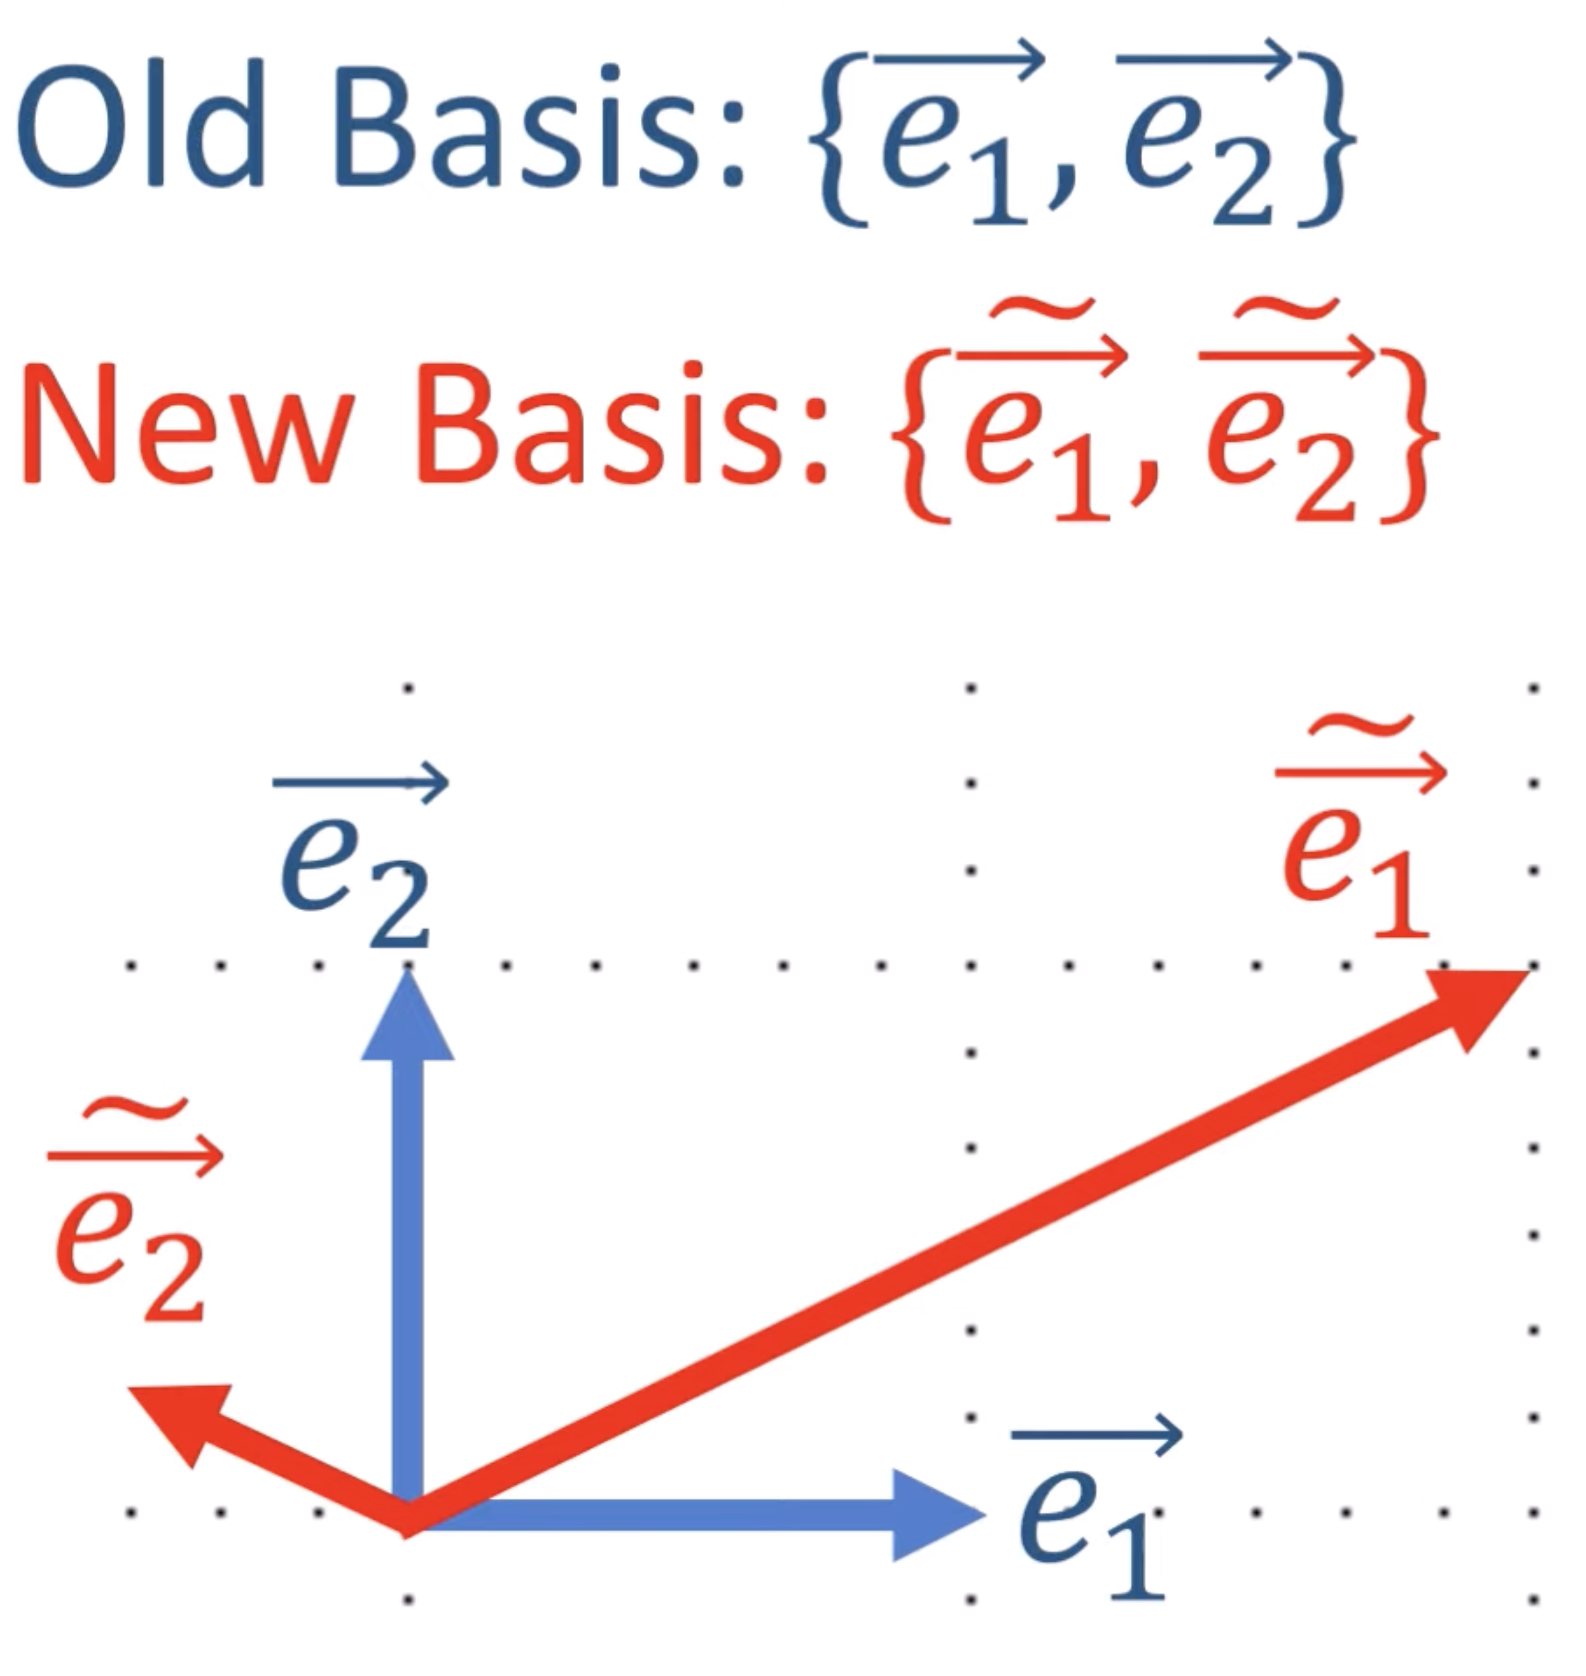
\includegraphics[width=0.25\textwidth]{Old_new_base_eigenchris}
    \caption{old and new basis vectors}
    \label{fig:old_new_base}
\end{figure}

\emph{Basis transformation:} The basis vectors of the new system expressed as a linear
combination of the basis vectors of the old system is considered a forward transformation.
The other direction is considered a backward transformation.\\

Here $F$ stands for $\underline{F}$orward transformation. Basis vectors are chosen to be
left multiplied to the transformation matrix, corresponding to summation via the first
index of the transformation matrix. Indices are chosen upper and lower to enable the
Einstein summation convention later on. Transformation indices are always from "north
west" to "south east":
\begin{equation}
    \label{eq:forward_trafo}
    \begin{array}{rcl}
        [\hdbtv{1} \quad \hdbtv{2}] & = &
        [\hdbv{1} \quad \hdbv{2}]
        \begin{bmatrix}
            F^{1~}_{~1} & F^{1~}_{~2} \\
            F^{2~}_{~1} & F^{2~}_{~2}
        \end{bmatrix} \\
        \noalign{\vskip10pt}
        \hdbtv{1} & = & F^{1~}_{~1}\hdbv{1} + F^{2~}_{~1}\hdbv{2}
        \quad \underset{\text{figure}~\ref{fig:old_new_base}}{=} \quad
        2 \hdbv{1} + 1 \hdbv{2} \\
        \hdbtv{2} & = & F^{1~}_{~2}\hdbv{1} + F^{2~}_{~2}\hdbv{2}
        \quad \underset{\text{figure}~\ref{fig:old_new_base}}{=} \quad
        -\frac{1}{2}\hdbv{1} + \frac{1}{4}\hdbv{2} \\
        \noalign{\vskip10pt}
        \Rightarrow \hdbtvc{j} & = &
        F^{k~}_{~j} \hdbvc{k} \quad\text{(summation convention)}
    \end{array}
\end{equation}

Here $B$ stands for $\underline{B}$ackward transformation:
\begin{equation}
    \label{eq:backward_trafo}
    \begin{array}{rcl}
        [\hdbv{1} \quad \hdbv{2}] & = &
        [\hdbtv{1} \quad \hdbtv{2}]
        \begin{bmatrix}
            B^{1~}_{~1} & B^{1~}_{~2} \\
            B^{2~}_{~1} & B^{2~}_{~2}
        \end{bmatrix} \\
        \noalign{\vskip10pt}
        \hdbv{1} & = & B^{1~}_{~1}\hdbtv{1} + B^{2~}_{~1}\hdbtv{2}
        \quad \underset{\text{figure}~\ref{fig:old_new_base}}{=} \quad
        \frac{1}{4} \hdbtv{1} + (-1) \hdbtv{2}\\
        \hdbv{2} & = & B^{1~}_{~2}\hdbtv{1} + B^{2~}_{~2}\hdbtv{2}
        \quad \underset{\text{figure}~\ref{fig:old_new_base}}{=} \quad
        \frac{1}{2}\hdbtv{1} + 2 \hdbtv{2} \\
        \noalign{\vskip10pt}
        \Rightarrow \hdbvc{i} & = &
        B^{j~}_{~i}\hdbtvc{j}\quad\text{(summation convention)}
    \end{array}
\end{equation}

Between $B$ and $F$ following relation holds:
\begin{equation}
    \label{eq:forward_backward_inverse}
    \begin{array}{rcl}
        B^{j~}_{~i} F^{k~}_{~j} & = & F^{k~}_{~j} B^{j~}_{~i}
        = \delta^k_i =
        \begin{cases}
            1, & \text{if}\ i = k \\
            0, & \text{if}\ i \neq k
        \end{cases} \\
        \text{full equation transposed:} & = &
        B^{i~}_{~j} F^{j~}_{~k} = \delta^i_k \\
        \noalign{\vskip10pt}
        \Rightarrow B & = & F^{-1} \quad\text{($B$ is the inverse of $F$)}
    \end{array}
\end{equation}


\newpage

\subsection{Vector Definition}

\begin{itemize}
  \item Vectors are \textcolor{red}{invariant} under a change of the coordinate system.
  \item Vector components are \textcolor{red}{not invariant} under a change of the
  coordinate system.
  \item Vectors can be defined for spaces of arbitrary dimension $n$. They form the vector
  space $V$ with their components $\in \mathbb{R}^n$.
  \item Not all vectors can be visualized as arrows (only easily done for vectors in
  Euclidean spaces).
\end{itemize}

Vectors are members of a vector space. A vector space needs four things:
\begin{enumerate}
  \item $V$: a set of vectors
  \item $S$: a set of scalars
  \item $+$: an operation to add vectors $\vec{v} + \vec{w} = 
  \overrightarrow{v+w}$
  \item $\cdot$: an operation to scale a vector by a scalar, e.g. $2\vec{v}$
\end{enumerate}
Vectors are basically things that can be added together and scaled by a factor. They are
written as colums of numbers of their components in the respective basis.

\begin{figure}[h]
  \centering
  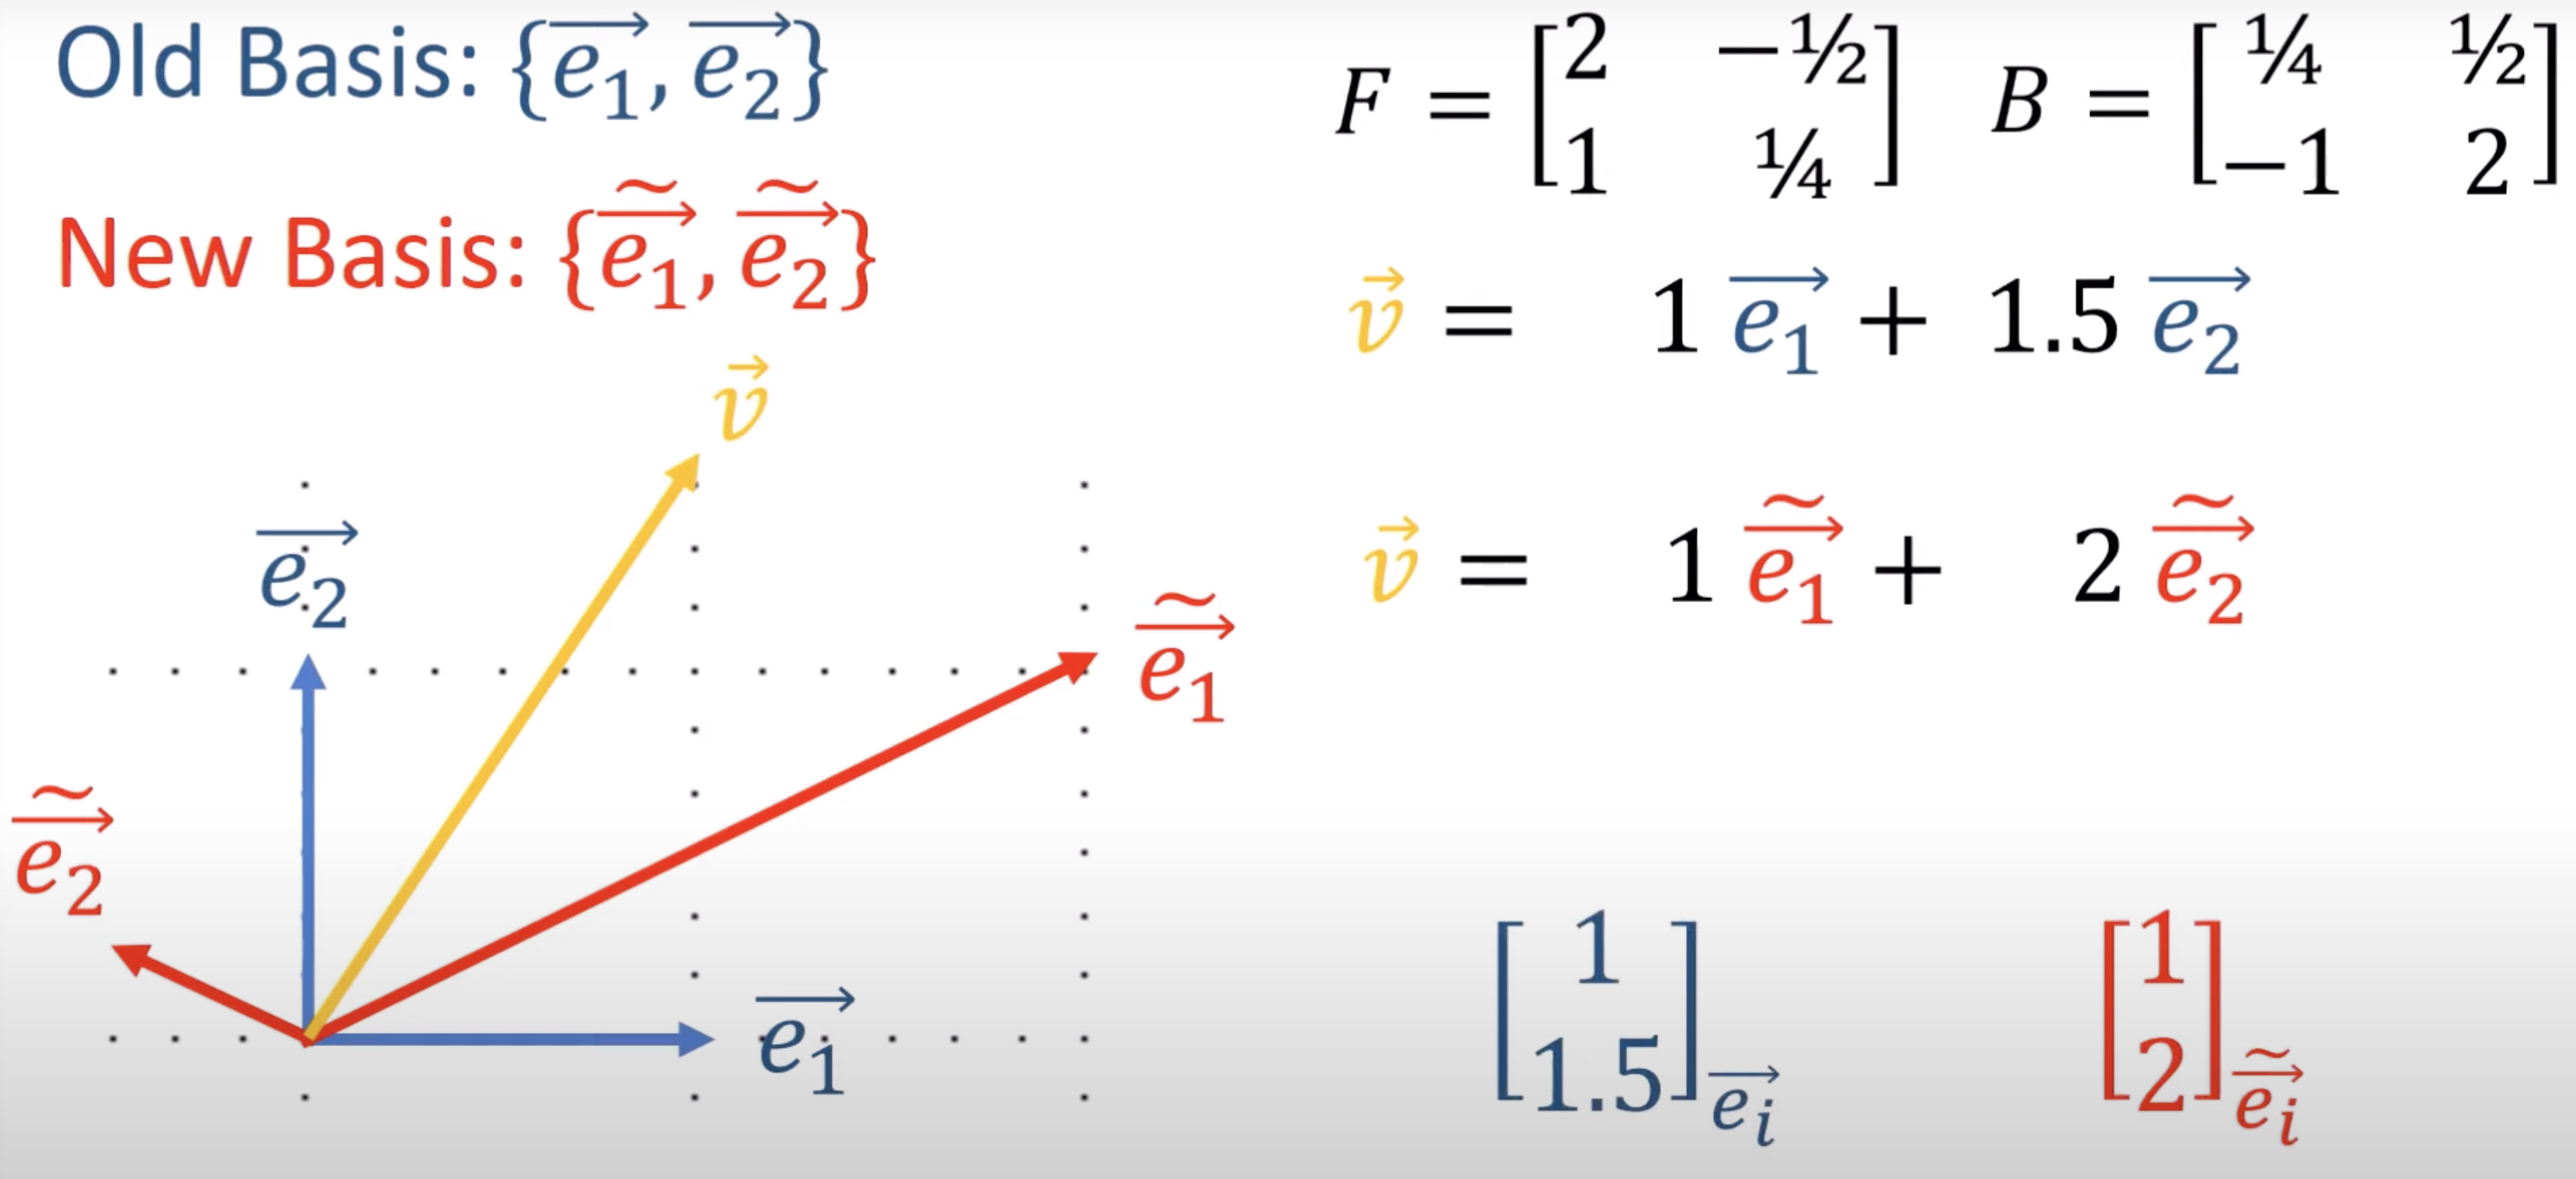
\includegraphics[width=0.7\textwidth]{vector_example_eigenchris}
  \caption{vector example in old and new system}
  \label{fig:vector_example_old_new_base}
\end{figure}

Vectors are formed by linear combinations of their basis vectors with the coordinates as
scaling coefficients of the corresponding basis vectors:
\begin{subequations}
  \begin{align}
    \label{eq:vector_def_old}
    \hdv & =  \sum\limits_i \hdvc{i} \hdbv{i} = \hdvc{i} \hdbvc{i}
    \quad\text{(summation convention)} \\
    \label{eq:vector_def_new}
    \hdv & = \sum\limits_i \hdtvc{i} \hdbtv{i} = \hdtvc{i} \hdbtvc{i}
    \quad\text{(summation convention)}
  \end{align}
\end{subequations}

Inserting the backward transformation (\ref{eq:backward_trafo}) in
(\ref{eq:vector_def_old}) and re-arranging the sums by exchanging the indices, we can get
the transformation rule of the vector components by comparing with
(\ref{eq:vector_def_new}). This yields the transformation rule for the vector components:
\begin{equation}
  \label{eq:vector_trafo_to_new}
  \begin{array}{rcl}
    \hdv & = & \hdvc{i} \hdbvc{i}
    = \hdvc{i} B^{j~}_{~i} \hdbtvc{j}
    = \hdvc{j} B^{i~}_{~j} \hdbtvc{i} \\
    \hdv & = & \hdtvc{i} \hdbtvc{i}
    \\ \noalign{\vskip10pt}
    \Rightarrow \hdtvc{i} & = & B^{i~}_{~j} \hdvc{j}
  \end{array}
\end{equation}

By inserting the forward transformation (\ref{eq:forward_trafo}) in
(\ref{eq:vector_def_new}) and re-arranging the sums, we can get the transformation rule of
the vector components by comparing with (\ref{eq:vector_def_old}). This yields the
transformation rule for the vector components in the other direction:
\begin{equation}
  \label{eq:vector_trafo_to_old}
  \begin{array}{rcl}
    \hdv & = & \hdvc{i} \hdbvc{i} \\
    \hdv & = & \hdtvc{i} \hdbtvc{i}
    = \hdtvc{i} F^{j~}_{~i}\hdbvc{j}
    = \hdtvc{j} F^{i~}_{~j}\hdbvc{i}\\
    \noalign{\vskip10pt}
    \Rightarrow \hdvc{i} & = &  F^{i~}_{~j} \hdtvc{j}
  \end{array}
\end{equation}

Summarizing the transformation rules for basis vectors and the respective vector
compontents we get:
\begin{equation}
  \label{eq:vector_trafo_overview}
  \begin{array}{rclrcl}
    \hdbtvc{i} & = &
    F^{j~}_{~i}\hdbvc{j} = \hdbvc{j} F^{j~}_{~i} \qquad\qquad
    \hdtvc{i} & = & B^{i~}_{~j} \hdvc{j} \\
    \hdbvc{i} & = &
    B^{j~}_{~i}\hdbtvc{j} = \hdbtvc{j} B^{j~}_{~i} \qquad\qquad
    \hdvc{i} & = &  F^{i~}_{~j} \hdtvc{j}
  \end{array}
\end{equation}

As can be seen, the basis vectors and their respective components transform with different
transformations. This transformation behaviour is called contravariant. Thus vectors are
contravariant tensors. \\
\begin{figure}[h]
  \centering
  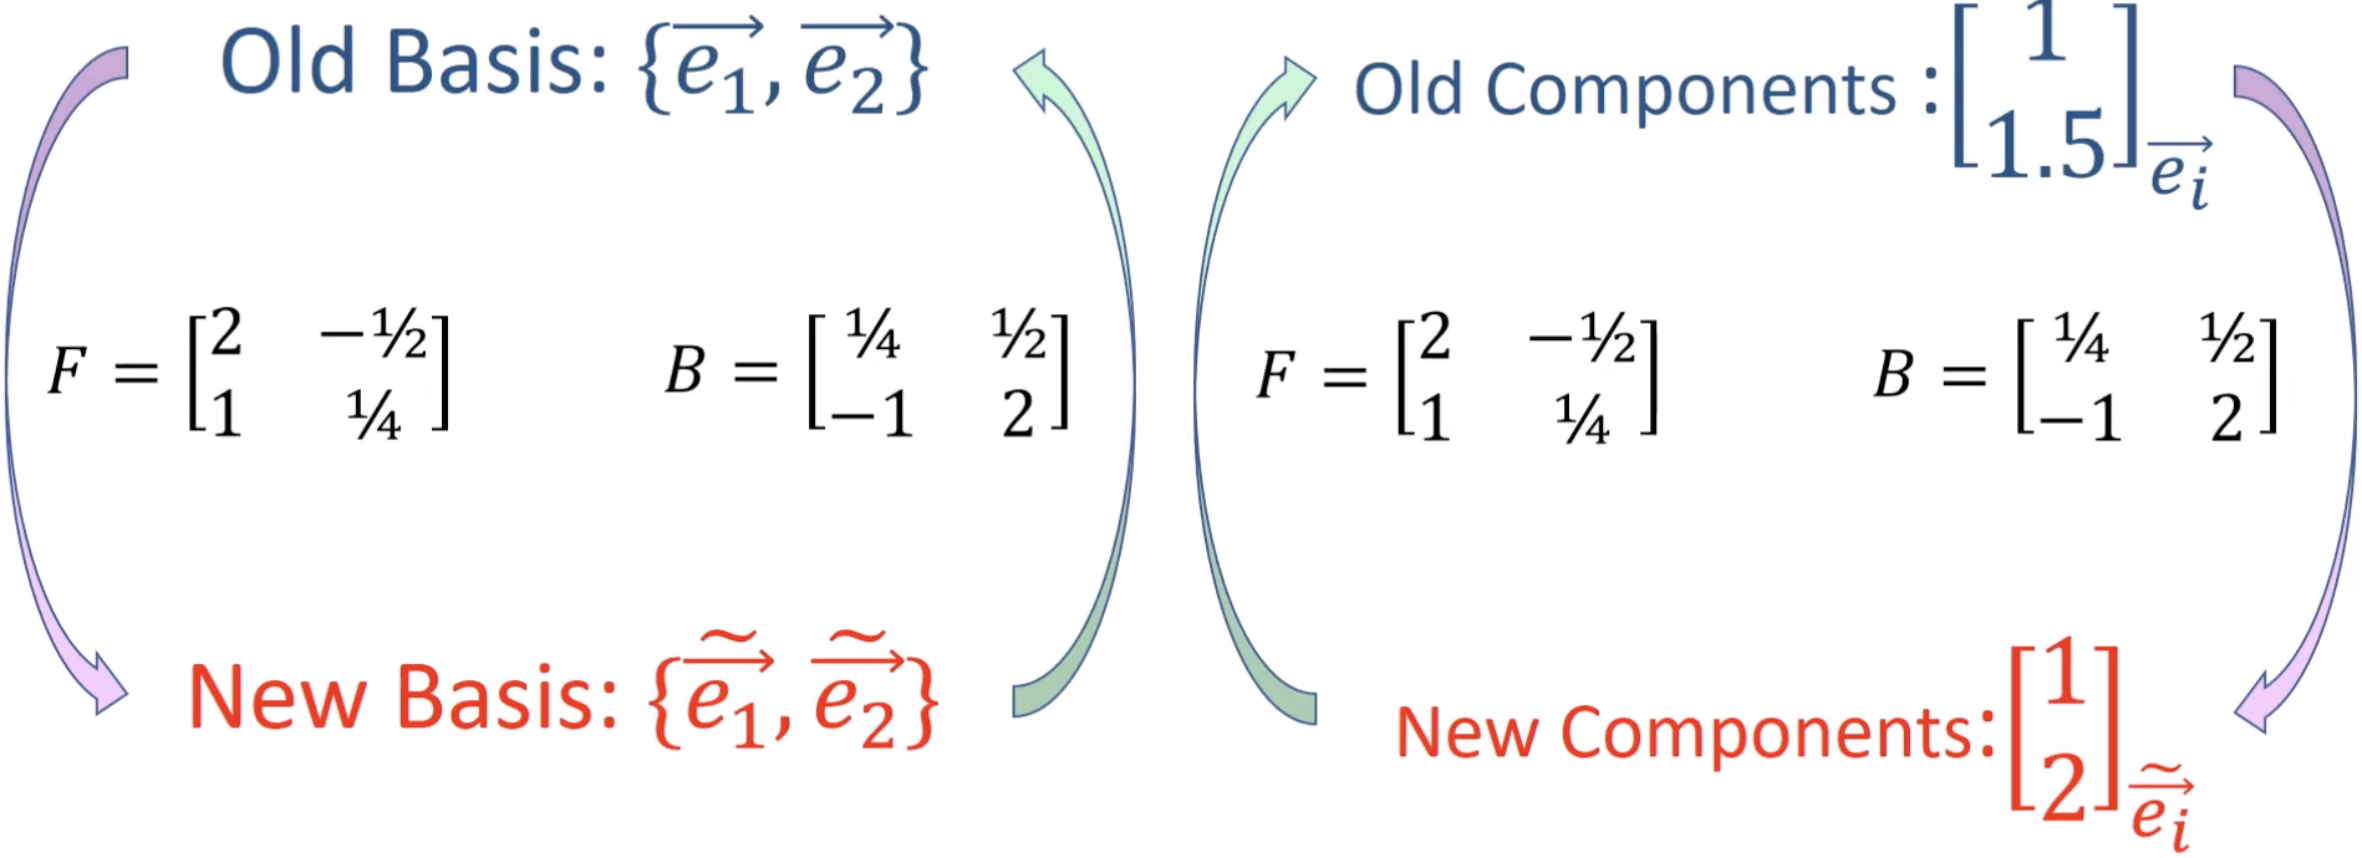
\includegraphics[width=0.65\textwidth]{Summary_transformations_eigenchris}
  \caption{Summary of transformations (example)}
  \label{fig:transformation_summary_example}
\end{figure}

For basis transformations the basis vectors are applied to the transformation matrix from
the left when written in matrix form, whereas vector components are multiplied from the
right with the transformation matrix. This can be seen in the index notation as well by
the position of the indices. Multiplication from the left corresponds to summation over
the first (or upstairs) index, while multiplication from the right corresponds to summation over the
second (or downstairs) index of the transformation matrix.

\newpage
\subsection{Covector Definition:}

Covectors and vectors are fundamentally different objects\footnote{Covectors can
"basically" be regarded as row vectors. However, only in an orthormal basis there is a
trivial link to column vector components. This is not true in the general case of
non-orthonormal basis vectors.}. Covectors are functions that take vectors as arguments.
They yield a scalar output $\alpha$ on a vector input $\vec{v}$:

\begin{equation}
    \alpha(\vec{v}) = \alpha_1 v^1 + \alpha_2 v^2 + \dots + \alpha_n v^n =
    \sum\limits_{i}\alpha_i \hdvc{i} 
\end{equation}

Covectors take an input from vector space $V$ and return a real number $\alpha$, i.e.
$\alpha: V \rightarrow \mathbb{R}$. Covectors have the linearity properties, i.e. they are
linear functions:

\begin{equation}
    \label{eq:covector_linearity}
    \begin{array}{rcl}
        \alpha(\textcolor{ForestGreen}{\vec{v}}+\textcolor{RoyalPurple}{\vec{w}}) & = &
        \alpha(\textcolor{ForestGreen}{\vec{v}})+\alpha(\textcolor{RoyalPurple}{\vec{w}}) \\
        \alpha(\textcolor{Goldenrod}{n}\textcolor{ForestGreen}{\vec{v}}) & = &
        \textcolor{Goldenrod}{n}\alpha(\textcolor{ForestGreen}{\vec{v}}) \\
        \alpha(\textcolor{Goldenrod}{n}\textcolor{ForestGreen}{\vec{v}}+
        \textcolor{YellowOrange}{m}\textcolor{RoyalPurple}{\vec{w}}) & = &
        \textcolor{Goldenrod}{n}\alpha(\textcolor{ForestGreen}{\vec{v}})+
        \textcolor{YellowOrange}{m}\alpha(\textcolor{RoyalPurple}{\vec{w}})
    \end{array}
\end{equation}

Covectors can also be viewed as elements of their own vector space $V^*$, i.e. they can be
scaled and added:

\begin{equation}
    \label{eq:covector_add_scale}
    \begin{array}{rcl}
        (n\alpha)(\hdv) & = &
        n\alpha(\hdv)\\
        (\beta + \gamma)(\hdv) & = &
        \beta(\hdv)+ \gamma(\hdv)
    \end{array}
\end{equation}

The vector space of contravariant vectors is defined by $(V,S,+,\cdot)$. The vector space
of covectors is defined by $(V^*,S,\textcolor{red}{+},\textcolor{red}{\cdot})$. The
covector operations $\textcolor{red}{+}$ and $\textcolor{red}{\cdot}$ are different from
the corresponding $+$ and $\cdot$ operations of vectors.

Covectors can be visualized as oriented stacks of lines of constant function value. When
the coordinates are vizualized as vectors they would provide a vector oriented as the
normal to the stack height lines:
\begin{figure}[h]
    \centering
    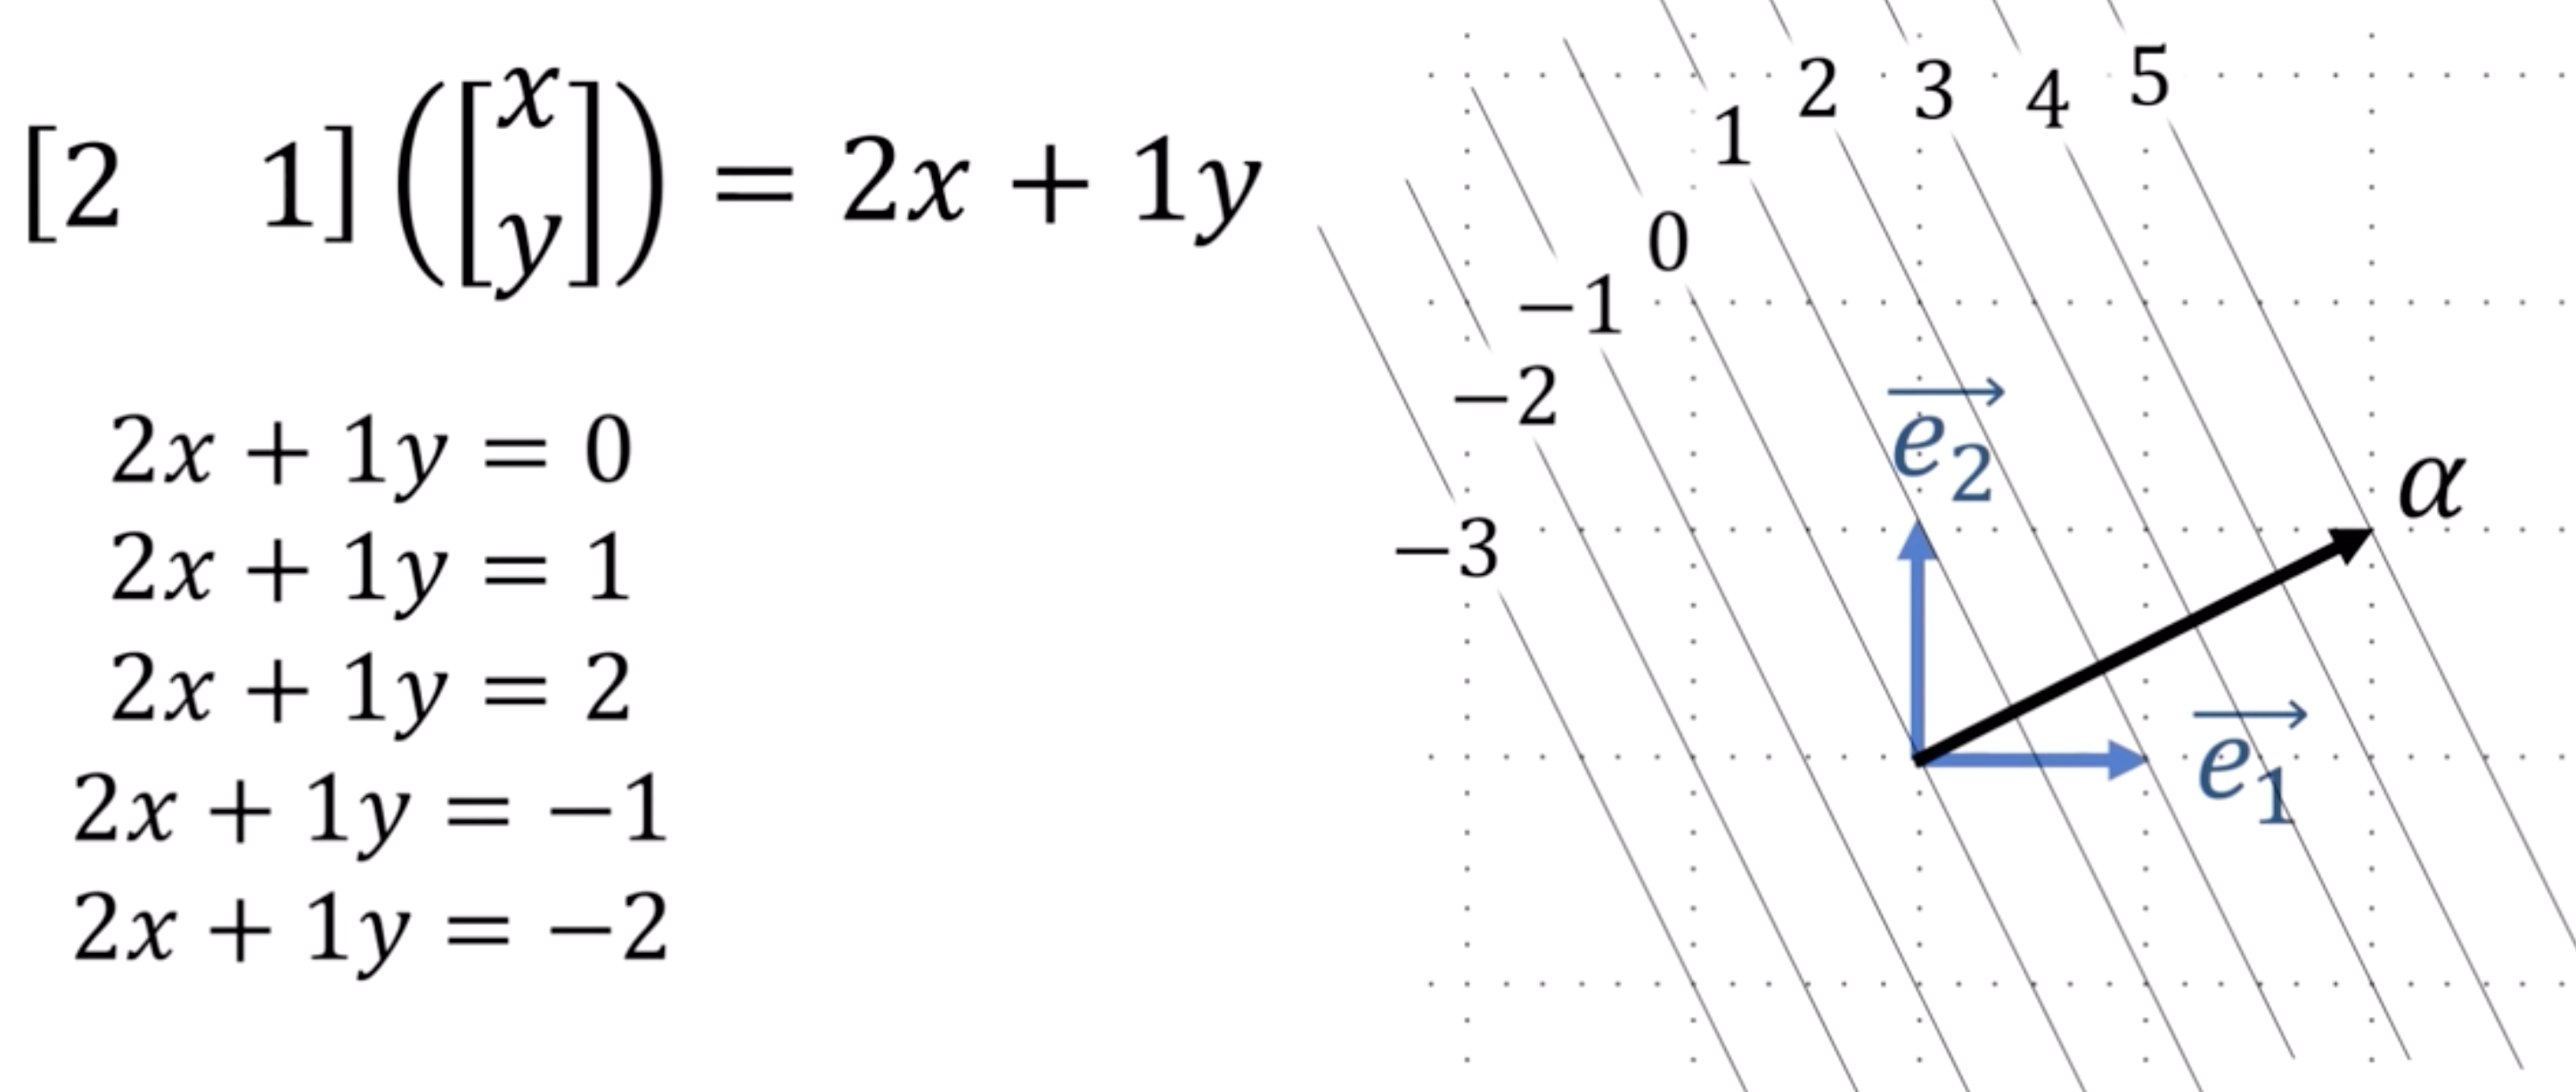
\includegraphics[width=0.7\textwidth]{Covector_as_oriented_stack_eigenchris}
    \caption{Example: covector visualized as lines of constant function value}
    \label{fig:covector_visualized}
\end{figure}

The function values returned by the covector can be visualized depending on the vectors
provided as arguments. The number of height lines pierced by the vector gives the returned
result:
\begin{figure}[h]
    \centering
    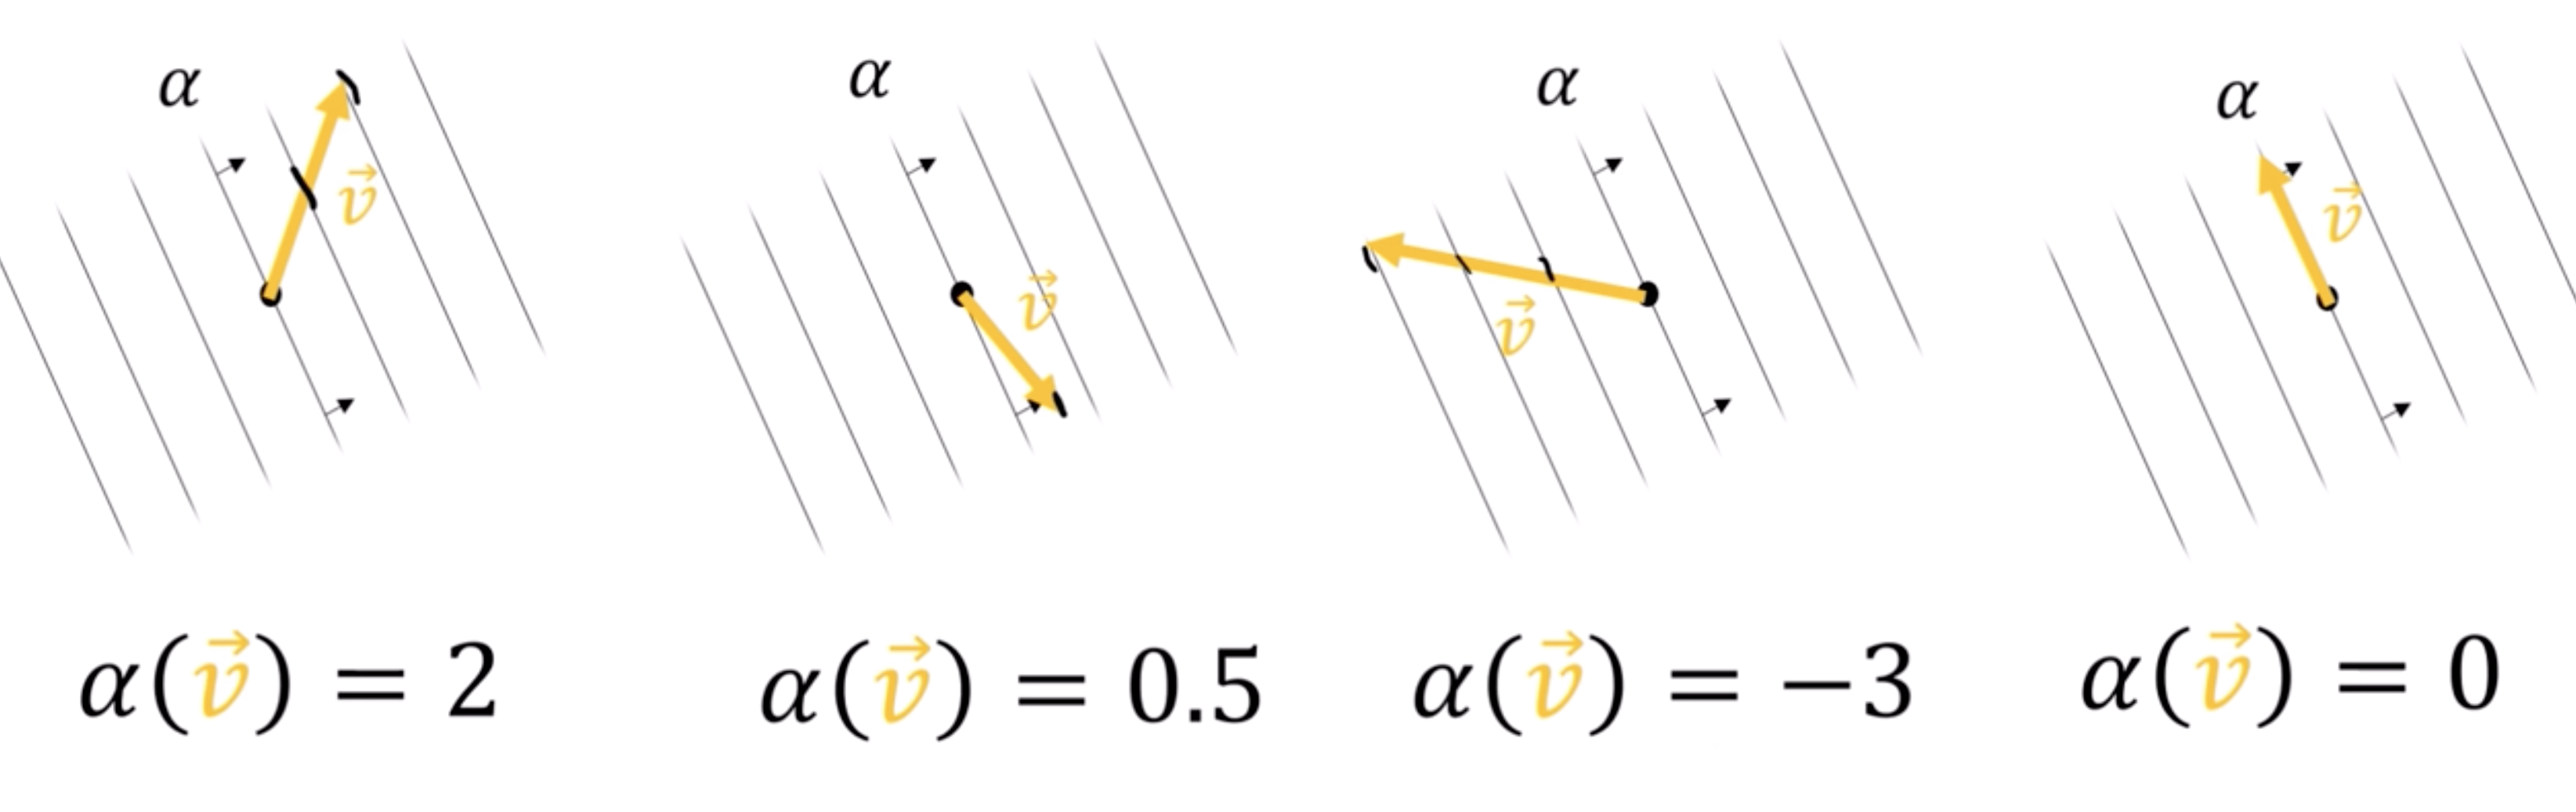
\includegraphics[width=0.9\textwidth]{Covector_return_values_eigenchris}
    \caption{Example: covector return values from given input vectors}
    \label{fig:covector_return_values}
\end{figure}

\begin{itemize}
    \item Covectors are \textcolor{red}{invariant} under a change of the coordinate
    system.
    \item Covector components are \textcolor{red}{not invariant} under a change of the
    coordinate system.
\end{itemize}

Covectors are functions $\alpha: V \rightarrow \mathbb{R}$ that take vectors as arguments.
Covectors don't live in the vector space $V$, but in $V^*$. Thus we cannot use basis
vectors like \{\hdbv{1}, \hdbv{2}\} to measure covectors directly. But still the basis
\{\hdbv{1}, \hdbv{2}\} can be used to derive a special covector basis \{\hdcbvc{1},
\hdcbvc{2}\} with the specific property:

\begin{equation}
    \label{eq:covec_vec_link}
    \begin{array}{rcl}
        \hdcbvc{i}(\hdbv{j}) & = &
        \delta^i_j = 
        \begin{cases}
            1, & \text{if}\ i = j \\
            0, & \text{if}\ i \neq j
        \end{cases} \\
        \noalign{\vskip10pt}
        \text{such that for the 2D case:}\qquad
        \hdcbvc{1}(\hdbv{1}) & = & 1 \qquad\qquad
        \hdcbvc{1}(\hdbv{2}) = 0 \\
        \hdcbvc{2}(\hdbv{1}) & = & 0 \qquad\qquad
        \hdcbvc{2}(\hdbv{2}) = 1
    \end{array}
\end{equation}

This effectively links the bases \hdcbvc{i} and \hdbv{i} and the vector spaces $V$ and
$V^*$, making $V^*$ the dual space of $V$. It enables us to use these covectors to find
the coordinates of arbitrary vectors of $V$ by applying these special covectors to them:

\begin{equation}
    \begin{array}{rcl}
        \label{eq:covec_application}
        \hdcbvc{1}(\hdv) & = &
        \hdcbvc{1}(\hdvc{1}\hdbv{1} + \hdvc{2}\hdbv{2})
        \underset{(\ref{eq:covector_linearity})}{=}
        \hdvc{1}\hdcbvc{1}(\hdbv{1}) + \hdvc{2}\hdcbvc{1}(\hdbv{2})
        \underset{(\ref{eq:covec_vec_link})}{=}
        \hdvc{1} \\
        \hdcbvc{2}(\hdv) & = &
        \hdcbvc{2}(\hdvc{1}\hdbv{1} + \hdvc{2}\hdbv{2})
        \underset{(\ref{eq:covector_linearity})}{=}
        \hdvc{1}\hdcbvc{2}(\hdbv{1}) + \hdvc{2}\hdcbvc{2}(\hdbv{2})
        \underset{(\ref{eq:covec_vec_link})}{=}
        \hdvc{2} \\
        \noalign{\vskip10pt}
        \Rightarrow \hdcbvc{i}(\hdv) & = & \hdvc{i}
    \end{array}
\end{equation}

This means we select a special covector basis that is aligned with our vector basis such
that each covector basis selects it's corresponding basis vector contribution exclusively:
\\

\begin{figure}[h]
    \centering
    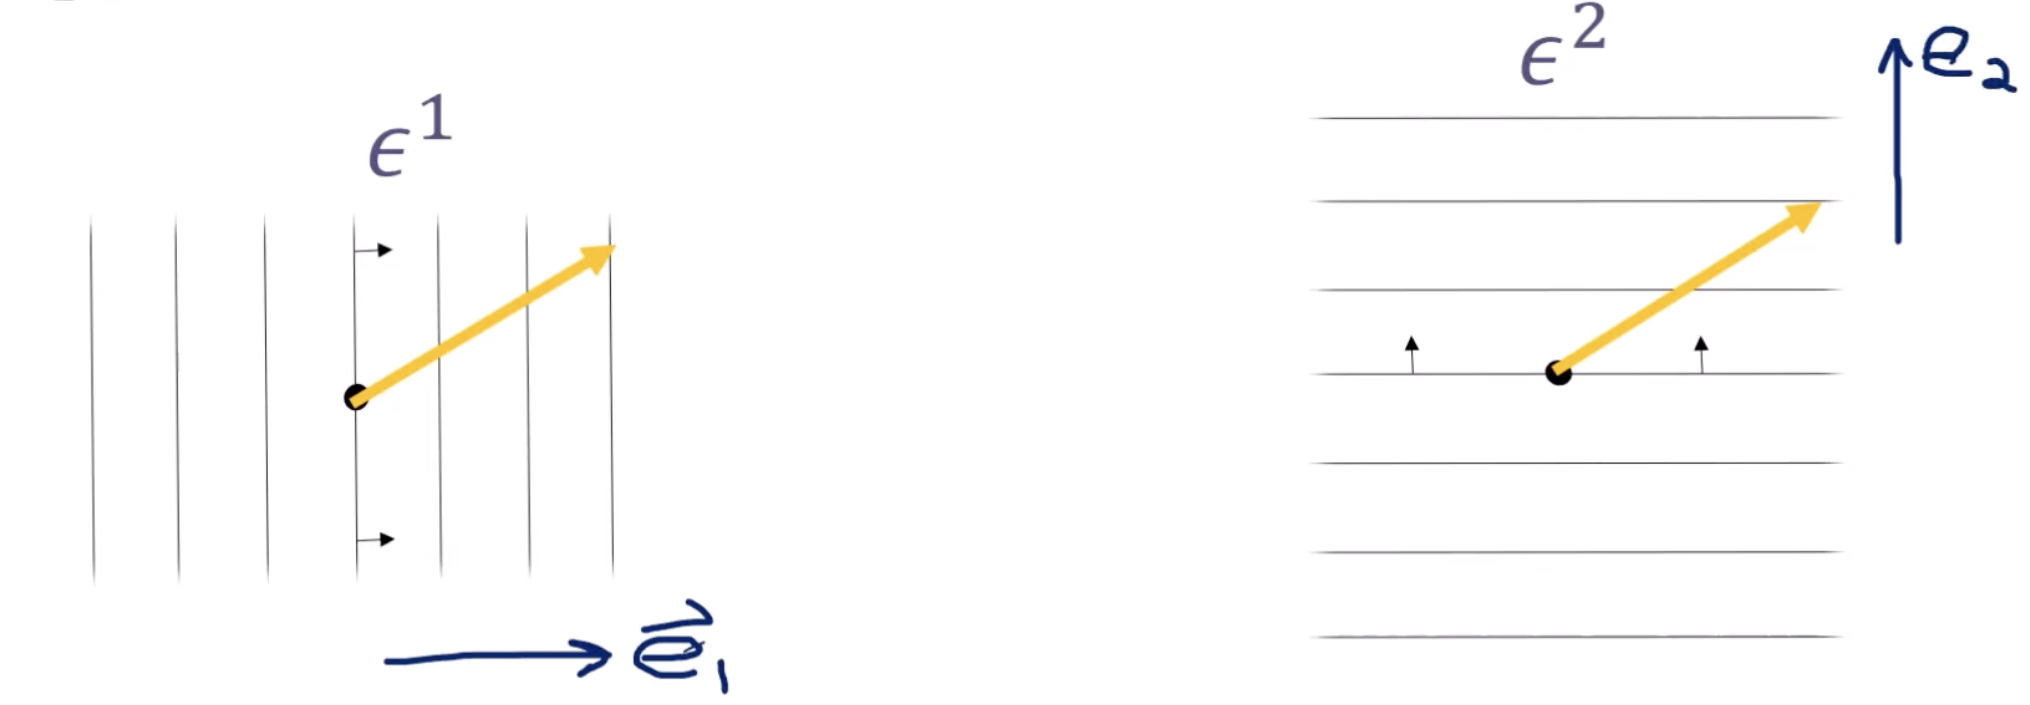
\includegraphics[width=0.8\textwidth]{Special_covector_bases_eigenchris}
    \caption{Example: specifically chosen covector basis}
    \label{fig:selected_covector_basis}
\end{figure}

If we now want to apply a general covector $\alpha$ to a vector $\hdv$ we can transform
the equations by defining the covector components in terms of our specially chosen
covector basis vectors \hdcbvc{1} and \hdcbvc{2}:

\begin{equation}
    \label{eq:covector_with_respect_to_old_basis} 
    \begin{array}{rcl}
        \alpha(\hdv) & = &
        \alpha(\hdvc{1}\hdbv{1} + \hdvc{2}\hdbv{2})
        \underset{(\ref{eq:covector_linearity})}{=}
        \hdvc{1}\alpha(\hdbv{1}) + \hdvc{2}\alpha(\hdbv{2}) \\
        & \underset{(\ref{eq:covec_application})}{=} &
        \hdcbvc{1}(\hdv)\alpha(\hdbv{1}) + \hdcbvc{2}(\hdv)\alpha(\hdbv{2}) \\
        \noalign{\vskip10pt}
        \text{defining}:\ \alpha(\hdbv{1}) & = & \alpha_1 \\
        \alpha(\hdbv{2}) & = & \alpha_2\\ 
        \noalign{\vskip10pt}
        \alpha(\hdv) & = &
        \alpha_1\hdcbvc{1}(\hdv) + \alpha_2\hdcbvc{2}(\hdv) \\
        & \underset{(\ref{eq:covector_add_scale})}{=} &
        (\alpha_1\hdcbvc{1} + \alpha_2\hdcbvc{2})(\hdv) \\
        \noalign{\vskip10pt}
        \Rightarrow \alpha & = & \alpha_1\hdcbvc{1} + \alpha_2\hdcbvc{2}
        = \alpha_i \hdcbvc{i}
    \end{array}
\end{equation}

Thus every covector can be expressed as a linear combination of our specifically chosen
covector basis. We call the basis \{\hdcbvc{1}, \hdcbvc{2}\} the ``dual basis'' of the vector
space $V^*$. Fig.~\ref{fig:arbitrary_covector_linearcombination} shows this graphically.\\

\begin{figure}[h]
    \centering
    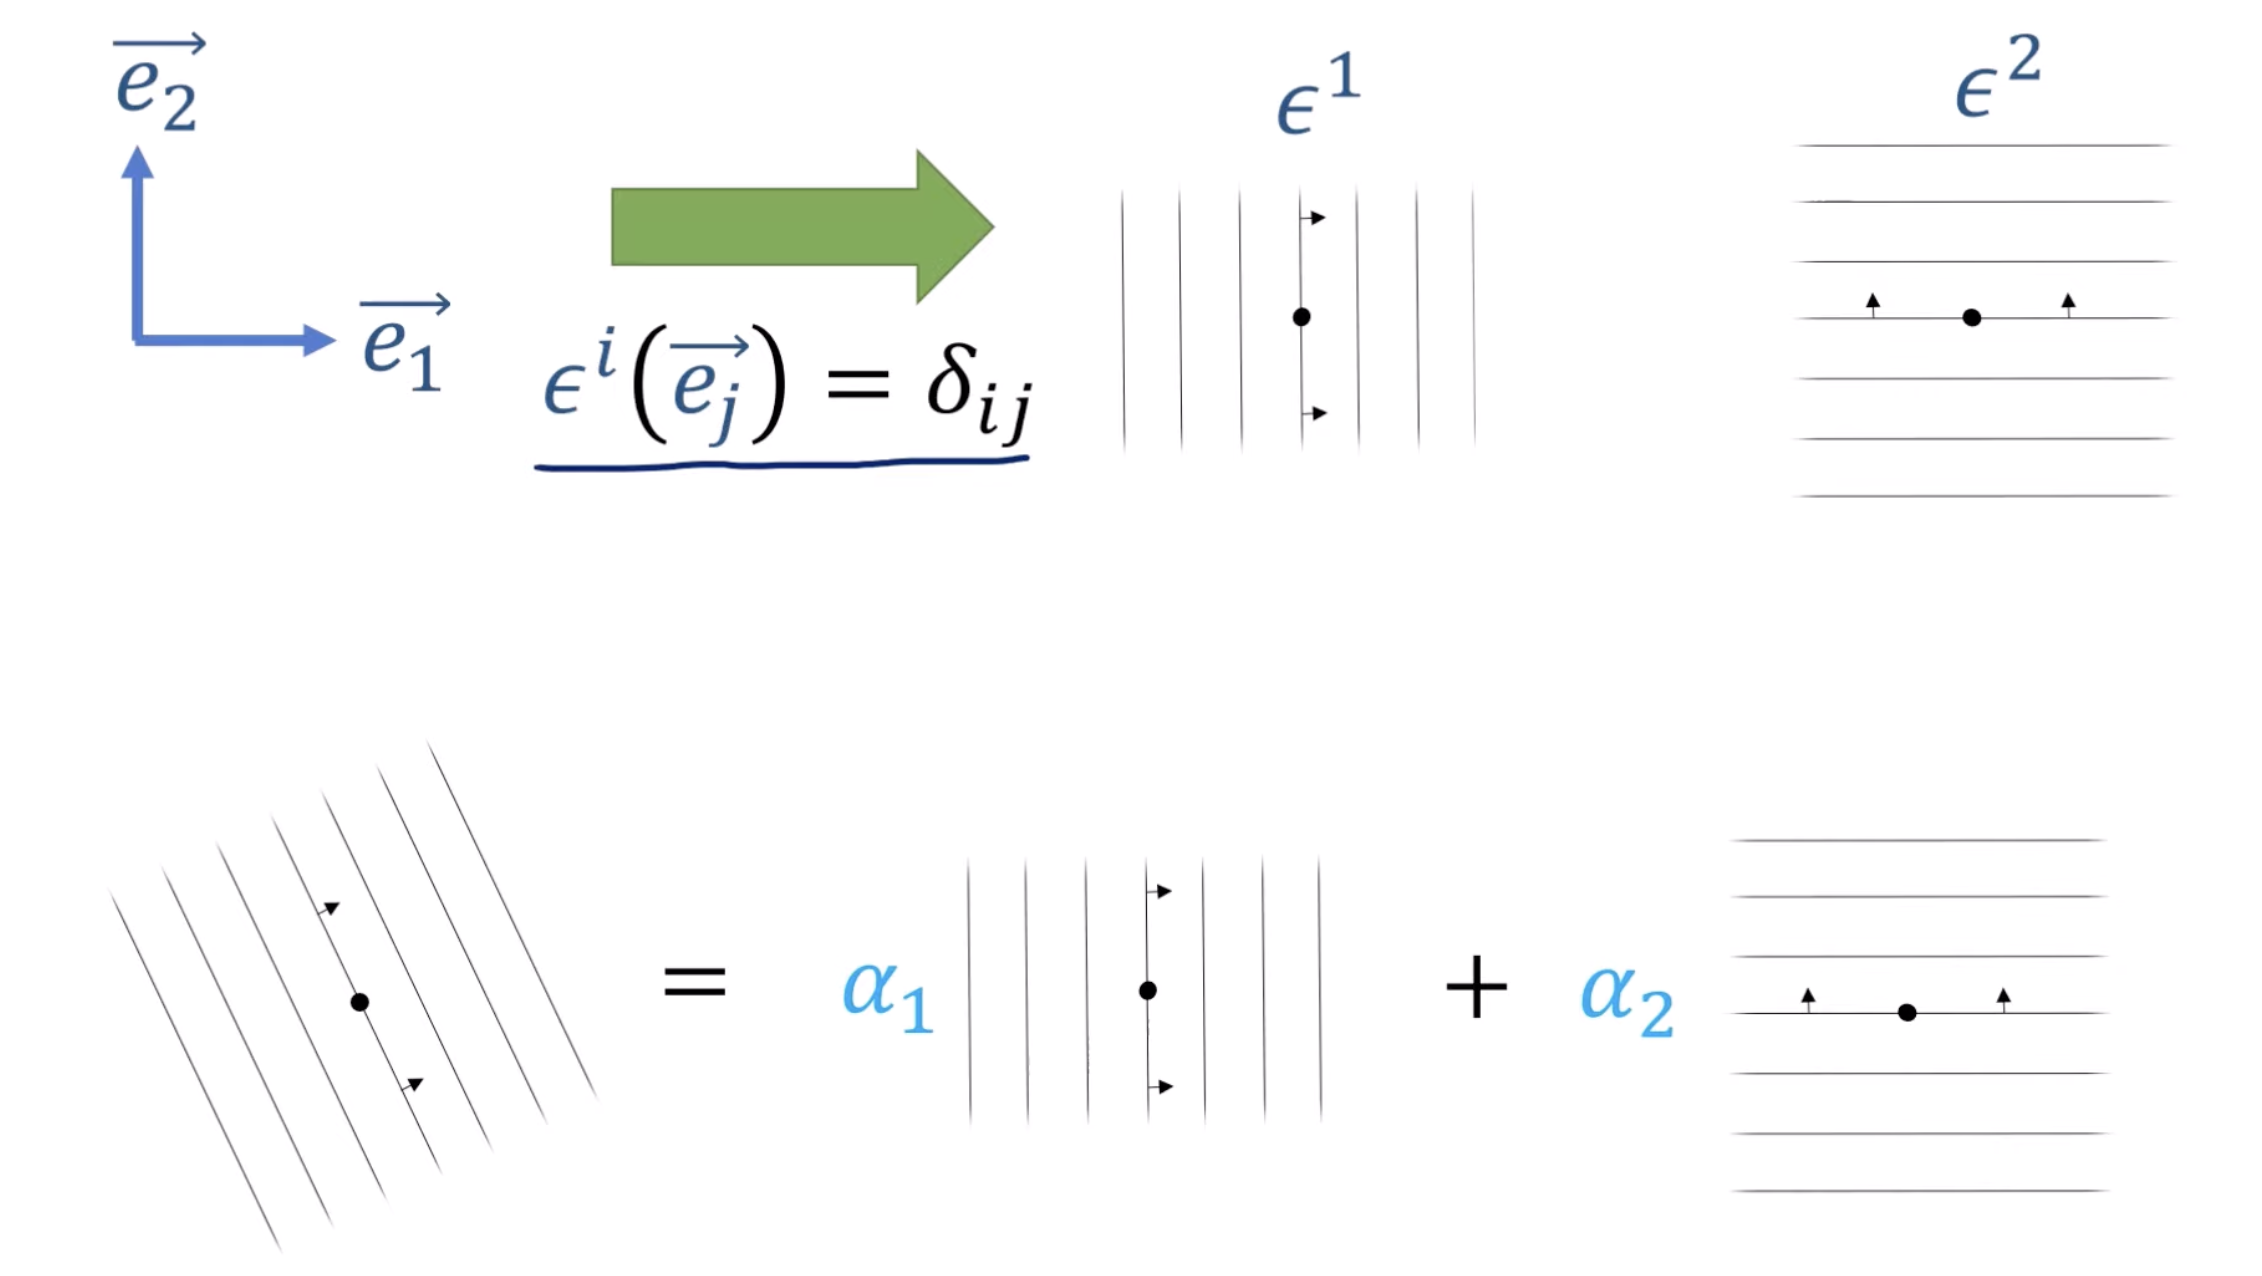
\includegraphics[width=0.6\textwidth]{Arbitray_covector_as_linearcombination_eigenchris}
    \caption{Arbitrary covector (lower row left) expressed as linear combination of the
    covector basis \{\hdcbvc{1}, \hdcbvc{2}\} after the dual basis has been derived from
    the vector basis.}
    \label{fig:arbitrary_covector_linearcombination}
\end{figure}

Of course we could also define an arbitray covector with respect to the vector basis in
the new system: The basis \{\hdbtv{1}, \hdbtv{2}\} can be used to derive a special
covector basis \{\hdcbtvc{1}, \hdcbtvc{2}\} with the specific property:
\begin{equation}
    \label{eq:covec_vec_link_new}
    \begin{array}{rcl}
        \hdcbtvc{i}(\hdbtv{j}) & = &
        \delta^i_j = 
        \begin{cases}
            1, & \text{if}\ i = j \\
            0, & \text{if}\ i \neq j
        \end{cases} \\
        \noalign{\vskip10pt}
        \text{such that for the 2D case:}\qquad
        \hdcbtvc{1}(\hdbtv{1}) & = & 1 \qquad\qquad
        \hdcbtvc{1}(\hdbtv{2}) = 0 \\
        \hdcbtvc{2}(\hdbtv{1}) & = & 0 \qquad\qquad
        \hdcbtvc{2}(\hdbtv{2}) = 1
    \end{array}
\end{equation}

This effectively links the bases \hdcbtvc{i} and \hdbtv{i} and the vector spaces $V$ and
$V^*$, making $V^*$ the dual space of $V$. It enables us to use these covectors to find
the coordinates of arbitrary vectors of $V$ by applying these special covectors to them:

\begin{equation}
    \begin{array}{rcl}
        \label{eq:covec_application_new}
        \hdcbtvc{1}(\hdv) & = &
        \hdcbtvc{1}(\hdtvc{1}\hdbtv{1} + \hdtvc{2}\hdbtv{2})
        \underset{(\ref{eq:covector_linearity})}{=}
        \hdtvc{1}\hdcbtvc{1}(\hdbtv{1}) + \hdtvc{2}\hdcbtvc{1}(\hdbtv{2})
        \underset{(\ref{eq:covec_vec_link_new})}{=}
        \hdtvc{1} \\
        \hdcbtvc{2}(\hdv) & = &
        \hdcbtvc{2}(\hdtvc{1}\hdbtv{1} + \hdtvc{2}\hdbtv{2})
        \underset{(\ref{eq:covector_linearity})}{=}
        \hdtvc{1}\hdcbtvc{2}(\hdbtv{1}) + \hdtvc{2}\hdcbtvc{2}(\hdbtv{2})
        \underset{(\ref{eq:covec_vec_link_new})}{=}
        \hdtvc{2} \\
        \noalign{\vskip10pt}
        \Rightarrow \hdcbtvc{i}(\hdv) & = & \hdtvc{i}
    \end{array}
\end{equation}

This leads to another dual basis specific for the basis vectors in the new
system as shown in equation~\ref{eq:covector_with_respect_to_new_basis}.

\begin{equation}
    \label{eq:covector_with_respect_to_new_basis} 
    \begin{array}{rcl}
        \alpha(\hdv) & = &
        \alpha(\hdtvc{1}\hdbtv{1} + \hdtvc{2}\hdbtv{2})
        \underset{(\ref{eq:covector_linearity})}{=}
        \hdtvc{1}\alpha(\hdbtv{1}) + \hdtvc{2}\alpha(\hdbtv{2}) \\
        & \underset{(\ref{eq:covec_application_new})}{=} &
        \hdcbtvc{1}(\hdv)\alpha(\hdbtv{1}) + \hdcbtvc{2}(\hdv)\alpha(\hdbtv{2}) \\
        \noalign{\vskip10pt}
        \text{defining:}\ \alpha(\hdbtv{1}) & = & \widetilde{\alpha_1} \\
        \alpha(\hdbtv{2}) & = & \widetilde{\alpha_2} \\ 
        \noalign{\vskip10pt}
        \alpha(\hdv) & = &
        \widetilde{\alpha_1}\hdcbtvc{1}(\hdv) + \widetilde{\alpha_2}\hdcbtvc{2}(\hdv) \\
        & \underset{(\ref{eq:covector_add_scale})}{=} &
        (\widetilde{\alpha_1}\hdcbtvc{1} + \widetilde{\alpha_2}\hdcbtvc{2})(\hdv) \\
        \noalign{\vskip10pt}
        \Rightarrow \alpha & = & \widetilde{\alpha_1}\hdcbtvc{1} + 
        \widetilde{\alpha_2}\hdcbtvc{2} =
        \widetilde{\alpha_i}\hdcbtvc{i}
    \end{array}
\end{equation}


Graphically fig.~\ref{fig:covectors_new_system} shows the covectors with respect to the
basis in the new system.\\

\begin{figure}[h]
    \centering
    \begin{subfigure}[b]{0.5175\textwidth}
        \centering
        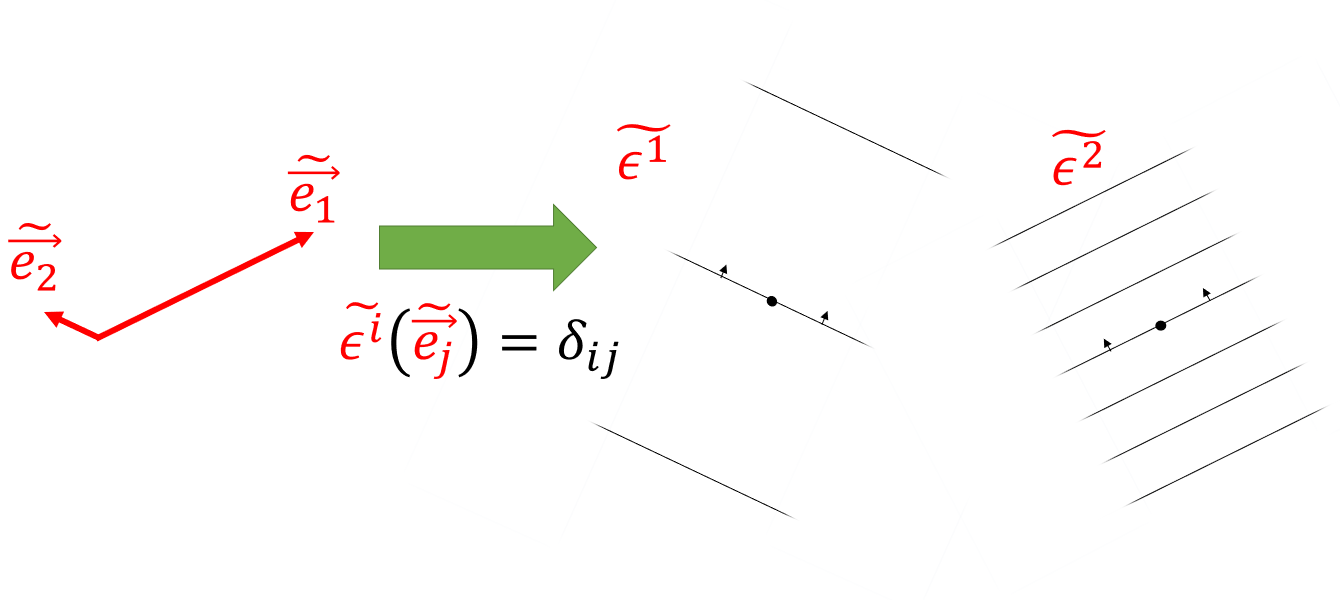
\includegraphics[width=\textwidth]{Covector_eigenchris1}
        \caption{Covector hight lines (new basis)}
    \end{subfigure}
    \hfill
    \begin{subfigure}[b]{0.45\textwidth}
        \centering
        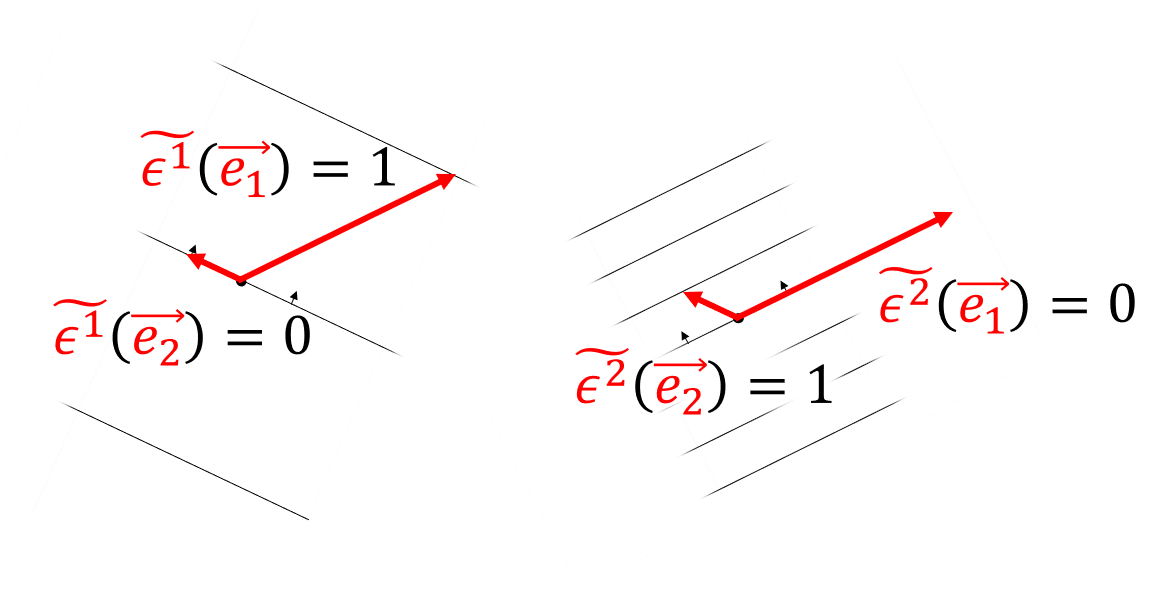
\includegraphics[width=\textwidth]{Covector_eigenchris2}
        \caption{Covector function (new basis)}
    \end{subfigure}
    \caption{Another dual covector basis expressed with respect to the basis in the new
    system}
    \label{fig:covectors_new_system}
\end{figure}

In order to derive the transformation rules for the the covector basis we use
\{\hdcbvc{j}\} as the old basis for $V^*$ and \{\hdcbtvc{i}\} as the new basis for $V^*$.
The new basis can be expressed by a linear combination of the old basis vectors using the
coefficients $Q^{i~}_{~j}$:
\begin{equation}
    \label{eq:covector_new_basis_as_linearcombination_in_old_basis}
    \hdcbtvc{i} = Q^{i~}_{~j}\hdcbvc{j}
\end{equation}

Using~(\ref{eq:covec_vec_link_new}) and
(\ref{eq:covector_new_basis_as_linearcombination_in_old_basis}) we can write:

\begin{equation}
    \label{eq:covector_transformation_rule} 
    \begin{array}{rcl}
        \hdcbtvc{i}(\hdbtv{k}) & = &
        Q^{i~}_{~j}\hdcbvc{j}(\hdbtv{k}) \\
        \delta^i_k &
        \underset{(\ref{eq:covec_vec_link_new}),(\ref{eq:forward_trafo})}{=} &
        Q^{i~}_{~j}\hdcbvc{j}(F^{l~}_{~k}\hdbv{l})
        \underset{(\ref{eq:covector_linearity})}{=}
        Q^{i~}_{~j} F^{l~}_{~k}\hdcbvc{j}(\hdbv{l}) \\
        \delta^i_k &
        \underset{(\ref{eq:covec_vec_link})}{=} &
        Q^{i~}_{~j} F^{l~}_{~k} \delta^j_l = Q^{i~}_{~j} F^{j~}_{~k} \\
        \text{comparing with~(\ref{eq:forward_backward_inverse}):\quad}
        Q^{i~}_{~j} & = & B^{i~}_{~j} \\
        \noalign{\vskip10pt}
        \text{inserting in~(\ref{eq:covector_new_basis_as_linearcombination_in_old_basis})}
        \Rightarrow \hdcbtvc{i} & = & B^{i~}_{~j}\hdcbvc{j}
    \end{array}
\end{equation}

This shows that covectors transform with the backward transformation from the old to the
new basis. Using the same approach it can be shown that:
\begin{equation}
    \label{eq:covector_transformation_rule_new}
    \begin{array}{rcl}
        \Rightarrow \hdcbvc{i} & = & F^{i~}_{~j}\hdcbtvc{j}
    \end{array}
\end{equation}

Summarizing the transformation rules for vectors and covectors we get:
\begin{equation}
    \label{eq:vector_covector_trafo_overview}
    \begin{array}{rclrcl}
      \hdbtvc{j} & = & F^{i~}_{~j}\hdbvc{i}
      \qquad\qquad
      \hdcbtvc{i} & = & B^{i~}_{~j} \hdcbvc{j} \\
      \hdbvc{j} & = & B^{i~}_{~j}\hdbtvc{i}
      \qquad\qquad
      \hdcbvc{i} & = &  F^{i~}_{~j} \hdcbtvc{j}
    \end{array}
  \end{equation}

The covector can be constructed from the basis in the old and new basis:
\begin{equation}
    \label{eq:covector_representation}
    \alpha = \alpha_i\hdcbvc{i} = \widetilde{\alpha_j}\hdcbtvc{j}
\end{equation}
By inserting the transformation rule~(\ref{eq:covector_transformation_rule})
or~(\ref{eq:covector_transformation_rule_new}) and comparing with the other part of the
equation~(\ref{eq:covector_representation}) we can get the transformation rules for the
covector components:
\begin{equation}
    \label{eq:covector_component_trafo}
    \begin{array}{rclrcl}
      \widetilde{\alpha_j} & = & F^{i~}_{~j}\alpha_i \\
      \alpha_j & = & B^{i~}_{~j}\widetilde{\alpha_i}
    \end{array}
  \end{equation}
  This means that covector components transform as the basis vectors do, i.e. with the
  forward transformation from the old to the new system and with the backward
  transformation from the new to the old system. This is called covariant transformation
  behaviour. For both cases the summation goes via the first index of the transformation
  matrix (equivalent to matrix multiplication from the left). \\

  Summing up everything so far we get:
  \begin{equation}
    \label{eq:summary_transformations}
    \boxed{
    \begin{array}{rclrcl}
      \hdbtvc{j} & = & F^{i~}_{~j}\hdbvc{i}
      \qquad \hfill
      \hdcbtvc{i} & = & B^{i~}_{~j} \hdcbvc{j}
      \quad\text{(\underline{contra}var.)} \\
      \hdbvc{j} & = & B^{i~}_{~j}\hdbtvc{i}
      \qquad\hfill
      \hdcbvc{i} & = &  F^{i~}_{~j} \hdcbtvc{j} \hfill \\
      \noalign{\vskip10pt}
      \text{with:}\quad \hdv & = & \hdvc{i} \hdbvc{i} = \hdtvc{j} \hdbtvc{j}
      \quad
      \alpha & = & \alpha_i\hdcbvc{i} = \widetilde{\alpha_j}\hdcbtvc{j}
      \hfill \\
      \noalign{\vskip10pt}
      \text{(\underline{contra}var.)}\quad
      \hdtvc{i} & = & B^{i~}_{~j} \hdvc{j}
      \qquad\hfill
      \widetilde{\alpha_j} & = & F^{i~}_{~j}\alpha_i
      \quad\text{(\underline{co}var.)}\hfill \\
      \hdvc{i} & = &  F^{i~}_{~j} \hdtvc{j}
      \qquad\hfill
      \alpha_j & = & B^{i~}_{~j}\widetilde{\alpha_i}\hfill
    \end{array}
    }
  \end{equation}

\newpage

\subsection{Linear Maps}

Linear maps take a vector as an input and produce a new vector as an output. Linear maps
don't transform the basis vectors. They just transform the input vectors into the output
vectors given in the same basis.\\

Linear maps shown as matrices contain the vector coordinates as columns they map copies of
the unit basis vectors ${\tiny\begin{bmatrix} 1 \\ 0\end{bmatrix}}$ and
${\tiny\begin{bmatrix} 0 \\ 1 \end{bmatrix}}$ to (see matrix multiplication with the
corresponding vector from the right side). The first column is the mapped value of the
first basis vector and the second column the mapped value of the second basis vector. In
general the $i^{th}$ column is the mapped value of the $i^{th}$ basis vector.\\

From a geometrical point of view linear maps are spactial transforms that keep gridlines
parallel, keep gridlines evenly spaced, and keep the origin stationary. That is linear
maps can stretch and rotate the input vectors, but they don't shift the origin.\\

From an abstract point of view linear maps do map vectors to vectors and have the
linearity properties, i.e. can be added and scaled. That means:
\begin{equation}
    \label{eq:linear_map_properties}
    \begin{array}{rcl}
        L: V \rightarrow  V &\text{or}& L: V \rightarrow W \\
        L(\textcolor{ForestGreen}{\vec{v}} + \textcolor{RoyalPurple}{\vec{w}}) & = &
        L(\textcolor{ForestGreen}{\vec{v}}) + L(\textcolor{RoyalPurple}{\vec{w}}) \\
        L(\textcolor{Goldenrod}{n}\textcolor{ForestGreen}{\vec{v}}) & = &
        \textcolor{Goldenrod}{n}L(\textcolor{ForestGreen}{\vec{v}}) 
    \end{array}
\end{equation}

We can derive the linear map and the resulting matrix multiplication of the vector
components directly from the linearity properties~(\ref{eq:linear_map_properties}):
\begin{equation}
    \label{eq:linear_map_derive_matrix_multiplication}
    \begin{array}{rcl}
        \textcolor{RoyalPurple}{\vec{w}} = L(\textcolor{Goldenrod}{\vec{v}}) & = &
        L(\hdvc{1}\hdbv{1} + \hdvc{2}\hdbv{2}) \\
        & \underset{(\ref{eq:linear_map_properties})}{=} &
        \hdvc{1}L(\hdbv{1}) + \hdvc{2}L(\hdbv{2})
    \end{array}
\end{equation}

Assuming $L: V\rightarrow V$, we can express the resulting vector in
\{\hdbv{1},\hdbv{2}\}:
\begin{equation}
    \label{eq:linear_map_derive_matrix_multiplication_2}
    \begin{array}{rcl}
        L(\hdbv{1}) & = & L^{1~}_{~1}\hdbv{1} + L^{2~}_{~1}\hdbv{2} \\
        L(\hdbv{2}) & = & L^{1~}_{~2}\hdbv{1} + L^{2~}_{~2}\hdbv{2} \\
        L(\hdbv{j}) & = & L^{k~}_{~j}\hdbv{k}
    \end{array}
\end{equation}
%Using~(\ref{eq:linear_map_derive_matrix_multiplication_2}) results in:
\begin{equation}
    \label{eq:linear_map_derive_matrix_multiplication_3}
    \begin{array}{rcl}
        \Rightarrow\textcolor{RoyalPurple}{\vec{w}} =
        L(\textcolor{Goldenrod}{\vec{v}}) & = &
        \hdvc{1}(L^{1~}_{~1}\hdbv{1} + L^{2~}_{~1}\hdbv{2}) +
        \hdvc{2}(L^{1~}_{~2}\hdbv{1} + L^{2~}_{~2}\hdbv{2}) \\
        & = & (L^{1~}_{~1}\hdvc{1}+ L^{1~}_{~2}\hdvc{2})\hdbv{1} +
        (L^{2~}_{~1}\hdvc{1} + L^{2~}_{~2}\hdvc{2})\hdbv{2} \\
        & = & \hspace{35pt}w^1\hspace{30pt}\hdbv{1} +
        \hspace{35pt}w^2\hspace{30pt}\hdbv{2} \\
        \noalign{\vskip10pt}
        w^1 & = & L^{1~}_{~1}\hdvc{1}+ L^{1~}_{~2}\hdvc{2} \\
        w^2 & = & L^{2~}_{~1}\hdvc{1} + L^{2~}_{~2}\hdvc{2} \\
        \noalign{\vskip10pt}
        \Rightarrow w^i & = &
        L^{i~}_{~j}\hdvc{j}
    \end{array}
\end{equation}


To figure out the transformation rules for linear maps we need to express the linear map
as an expansion in the new basis to see how the new basis vector are mapped:
\begin{equation}
    \label{eq:linear_map_transform_to_new_basis}  
    \begin{array}{rcl}
        \widetilde{L^{l~}_{~i}}\hdbtv{l} & = & L(\hdbtv{i}) \\
        & \underset{(\ref{eq:forward_trafo})}{=} &
        L(F^{j~}_{~i}\hdbv{j}) \underset{(\ref{eq:linear_map_properties})}{=}
        F^{j~}_{~i}L(\hdbv{j}) \\
        & \underset{(\ref{eq:linear_map_derive_matrix_multiplication_2})}{=} &
        F^{j~}_{~i}L^{k~}_{~j}\hdbv{k} \underset{(\ref{eq:backward_trafo})}{=}
        F^{j~}_{~i}L^{k~}_{~j} B^{l~}_{~k}\hdbtv{l} \\
        \widetilde{L^{l~}_{~i}}\hdbtv{l} & = &
        B^{l~}_{~k} L^{k~}_{~j} F^{j~}_{~i} \hdbtv{l} \\
        \noalign{\vskip10pt}
        \Rightarrow \widetilde{L^{l~}_{~i}} & = &
        B^{l~}_{~k} L^{k~}_{~j} F^{j~}_{~i}
    \end{array}
\end{equation}

To figure out the transformation to the old basis we can use the fact that the forward and
the backward transform are inverses of each other~(\ref{eq:forward_backward_inverse}). By
multiplying~(\ref{eq:linear_map_transform_to_new_basis}) from the left with the forward
transformation matrix $F^{s~}_{~l}$ and from the right with the backward transformation
matrix $B^{i~}_{~t}$we get:
\begin{equation}
    \label{eq:linear_map_transform_to_old_basis}  
    \begin{array}{rcl}
        \widetilde{L^{l~}_{~i}} & = & B^{l~}_{~k} L^{k~}_{~j} F^{j~}_{~i} \\
        F^{s~}_{~l}\widetilde{L^{l~}_{~i}}B^{i~}_{~t} & = &
        F^{s~}_{~l}B^{l~}_{~k} L^{k~}_{~j} F^{j~}_{~i} B^{i~}_{~t} \\
        & = & \delta^s_k L^{k~}_{~j} \delta^j_t = L^{s~}_{~t} \\
        \noalign{\vskip10pt}
        \Rightarrow L^{s~}_{~t} & = & F^{s~}_{~l}\widetilde{L^{l~}_{~i}}B^{i~}_{~t}  
    \end{array}
\end{equation}

\textbf{To sum up everything up to here:}\\

\textcolor{red}{\underline{Contra}variant (1,0)-tensors} transform like this (basis /
components) - the components can be written as column vectors and are multiplied to the
matrix from the right:
\begin{equation}
    \begin{array}{rcl}
        \hdcbtvc{i} & = & B^{i~}_{~j} \hdcbvc{j} \\
        \hdcbvc{i} & = & F^{i~}_{~j}  \hdcbtvc{j}
    \end{array}
    \qquad
    \begin{array}{rcl}
        \hdtvc{i} & = & B^{i~}_{~j} \hdvc{j} \\
        \hdvc{i} & = & F^{i~}_{~j}  \hdtvc{j}
    \end{array}
\end{equation}

\textcolor{red}{\underline{Co}variant (0,1)-tensors} transform like this (basis /
components) - the components can be written as row vectors and are multiplied to the
matrix from the left:
\begin{equation}
    \begin{array}{rcl}
        \hdbtv{j} & = & \hdbv{i}  F^{i~}_{~j} \\
        \hdbv{j} & = & \hdbtv{i} B^{i~}_{~j} 
    \end{array}
    \qquad
    \begin{array}{rcl}
        \widetilde{{\alpha_j}} & = & {\alpha_i} F^{i~}_{~j}  \\
        {\alpha_j} & = & \widetilde{{\alpha_i}} B^{i~}_{~j}
    \end{array}
\end{equation}

\textcolor{red}{Linear maps are (1,1)-tensors}, i.e. they have a vector and a covector
part and transform like this - the matrix of the coefficients of the linear map is
multiplied from the left and the right with the respective forward or backward
transformation matrices:
\begin{equation}
    \begin{array}{rcl}
        \textcolor{red}{\widetilde{L^{i~}_{~j}}} & = &
        B^{i~}_{~k} \textcolor{MidnightBlue}{L^{k~}_{~l}} F^{l~}_{~j} \\
        \textcolor{MidnightBlue}{L^{i~}_{~j}} & = &
        F^{i~}_{~k} \textcolor{red}{\widetilde{L^{k~}_{~l}}} B^{l~}_{~j}
    \end{array}
\end{equation}

\newpage

\subsection{Metric Tensor}

The length of a vector in an arbitrary coordinate system is defined by its norm which in
turn is defined by the scalar product:
\begin{equation}
    \begin{array}{rcl}
        \|\vec{v}\|^2 & = & \vec{v} \cdot \vec{v} \\
        \noalign{\vskip10pt}
        & = & (v^1 \hdbv{1} + v^2 \hdbv{2}) \cdot (v^1 \hdbv{1} + v^2 \hdbv{2}) \\ 
        & = & (v^1)^2(\hdbv{1}\cdot\hdbv{1}) + v^1 v^2 (\hdbv{1}\cdot\hdbv{2}) +
               v^2 v^1 (\hdbv{2}\cdot\hdbv{1}) +(v^2)^2(\hdbv{2}\cdot\hdbv{2}) \\
        & = & (v^1)^2(\hdbv{1}\cdot\hdbv{1}) + 2 v^1 v^2 (\hdbv{1}\cdot\hdbv{2}) +
              (v^2)^2(\hdbv{2}\cdot\hdbv{2}) \\
        \noalign{\vskip10pt}
        & = & (\tilde{v}^1)^2(\hdbtv{1}\cdot\hdbtv{1}) + 2 \tilde{v}^1 \tilde{v}^2 (\hdbtv{1}\cdot\hdbtv{2}) +
              (\tilde{v}^2)^2(\hdbtv{2}\cdot\hdbtv{2})              
    \end{array}
\end{equation}

In orthogonal coordinate systems the mixed products $(\hdbv{1}\cdot\hdbv{2})$ and
$(\hdbtv{1}\cdot\hdbtv{2})$ are equal to $0$, but in the more general non-orthogonal case
these terms do not disappear. \\

The scalar product can be written in component form based on the summation convention with
an implied summation over $i$ and $j$ as
\begin{equation}
    \begin{array}{rcl}
        \|\vec{v}\|^2 = \vec{v} \cdot \vec{v} & = & (v^i \hdbv{i}) \cdot (v^j \hdbv{j})
                        = v^i v^j (\hdbv{i}\cdot\hdbv{j})
                        = v^i v^j g_{ij} \\
        & = & (\tilde{v}^i \hdbtv{i}) \cdot (\tilde{v}^j \hdbtv{j})
          = \tilde{v}^i \tilde{v}^j (\hdbtv{i}\cdot\hdbtv{j})
          = \tilde{v}^i \tilde{v}^j \tilde{g}_{ij}
    \end{array}
\end{equation}
Here $g$ is the metric tensor given in coordinates of the old and new system respectively.
It's components are defined by the scalar products:
\begin{equation}
    \begin{array}{rcl}
        g_{ij} & = & (\hdbv{i}\cdot\hdbv{j}) \\
        \tilde{g}_{ij} & = & (\hdbtv{i}\cdot\hdbtv{j})
    \end{array}
\end{equation}
In component form it can be written as a symmetric matrix, because the sequence of
arguments does not influence the result of the dot product.
\begin{equation}
    \begin{array}{rcl}
        g_{\hdbv{i}}& = &
        \prescript{}{}{\begin{bmatrix}
            \hdbv{1}\cdot\hdbv{1} & \hdbv{1}\cdot\hdbv{2} \\
            \hdbv{2}\cdot\hdbv{1} & \hdbv{2}\cdot\hdbv{2} 
        \end{bmatrix}_{\hdbv{i}}} \\
        \noalign{\vskip10pt}
        g_{\hdbtv{i}}& = &
        \prescript{}{}{\begin{bmatrix}
            \hdbtv{1}\cdot\hdbtv{1} & \hdbtv{1}\cdot\hdbtv{2} \\
            \hdbtv{2}\cdot\hdbtv{1} & \hdbtv{2}\cdot\hdbtv{2} 
        \end{bmatrix}_{\hdbtv{i}}}
    \end{array}
\end{equation}

All dot products can be computed in an arbitrary basis system by using the metric
tensor:
\begin{equation}
    \label{eq:scalar_product_definition}
    \begin{array}{rclrcl}
        \vec{v} \cdot \vec{v} & = & \|\vec{v}\|^2 & = & v^i v^j g_{ij} = \tilde{v}^i \tilde{v}^j \tilde{g}_{ij} \\
        \vec{w} \cdot \vec{w} & = & \|\vec{w}\|^2 & = & w^i w^j g_{ij} = \tilde{w}^i \tilde{w}^j \tilde{g}_{ij} \\
        \vec{v} \cdot \vec{w} & = & \|\vec{v}\|  \|\vec{w}\| \cos(\theta) & = & v^i w^j g_{ij}  = \tilde{v}^i \tilde{w}^j \tilde{g}_{ij}
    \end{array}
\end{equation}
To show that the last formula in equation (\ref{eq:scalar_product_definition}) is correct,
consider figure~\ref{fig:angle_between_arbitrary_vectors}.
\begin{figure}[h]
    \centering
    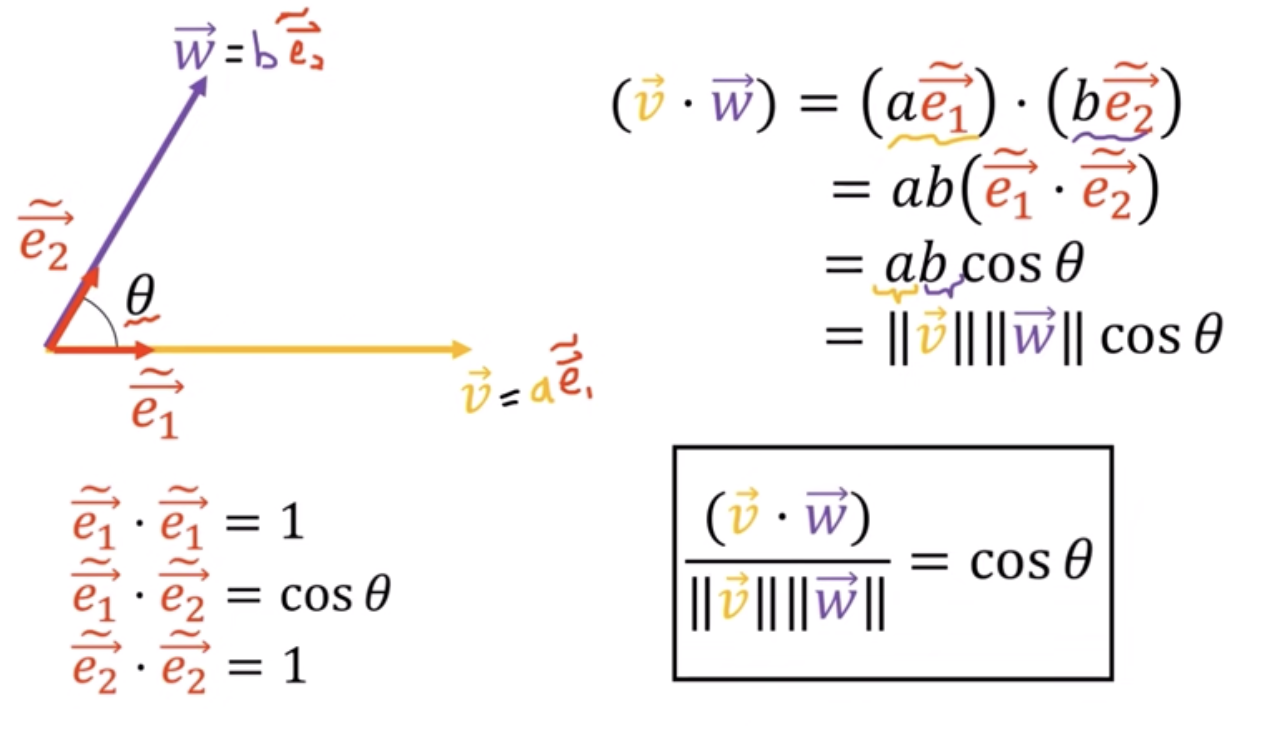
\includegraphics[width=0.6\textwidth]{Angle_between_vectors_dotproduct}
    \caption{Angle $\theta$ between two arbitrary vectors.}
    \label{fig:angle_between_arbitrary_vectors}
\end{figure} \\

To check how the metric tensor transforms, we use the formulation of the metric tensor in
the new system and transform it by replacing the tilde-components by expressing them in
the old system via the definitions of the forward transform given by
equation~(\ref{eq:vector_trafo_overview}):

\begin{equation}
    \begin{array}{rcl}
        \tilde{g}_{ij} & = & \hdbtv{i} \cdot \hdbtv{j} \\
                       & = & (F^{k~}_{~i}\hdbv{k}) \cdot (F^{l~}_{~j}\hdbv{l}) \\
                       & = & F^{k~}_{~i}  F^{l~}_{~j} (\hdbv{k} \cdot \hdbv{l}) \\
        \Rightarrow\tilde{g}_{ij} & = & F^{k~}_{~i}  F^{l~}_{~j} {g}_{kl} \\
        \noalign{\vskip10pt}
        g_{kl} & = & \hdbv{k} \cdot \hdbv{l} \\
        & = & (B^{i~}_{~k}\hdbtv{i}) \cdot (B^{j~}_{~l}\hdbtv{j}) \\
        & = & B^{i~}_{~k} B^{j~}_{~l} (\hdbtv{i} \cdot \hdbtv{j}) \\
        \Rightarrow g_{kl} & = & B^{i~}_{~k} B^{j~}_{~l}  \tilde{g}_{ij}
    \end{array}
\end{equation} \\

\textcolor{red}{Metric tensors are (0,2)-tensors}, because they transform with covariant
transformation behaviour using two transformations for change from one system to another.
This is also suggested by using lower indices for the metric tensor components. \\


\newpage

\subsection{Transformation laws of arbitrary tensors}
Let's review the defintion 1 of a tensor from the front page: \emph{``A tensor is an
object that is invariant under a change of coordinates, and has components that change in
a special, predictable way under a change of coordinates.''} \\

\textbf{To sum up everything up to here:}\\

\textcolor{red}{\underline{Contra}variant (1,0)-tensors} transform like this (basis /
components) - the components can be written as column vectors and are multiplied to the
matrix from the right (i.e. summation over the second index):
\begin{equation}
    \begin{array}{rcl}
        \hdcbtvc{i} & = & B^{i~}_{~j} \hdcbvc{j} \\
        \hdcbvc{i} & = & F^{i~}_{~j}  \hdcbtvc{j}
    \end{array}
    \qquad
    \begin{array}{rcl}
        \hdtvc{i} & = & B^{i~}_{~j} \hdvc{j} \\
        \hdvc{i} & = & F^{i~}_{~j}  \hdtvc{j}
    \end{array}
\end{equation}

\textcolor{red}{\underline{Co}variant (0,1)-tensors} transform like this (basis /
components) - the components can be written as row vectors and are multiplied to the
matrix from the left (i.e. summation over the first index):
\begin{equation}
    \begin{array}{rcl}
        \hdbtv{j} & = & \hdbv{i}  F^{i~}_{~j} = F^{i~}_{~j} \hdbv{i}\\
        \hdbv{j} & = & \hdbtv{i} B^{i~}_{~j} = B^{i~}_{~j} \hdbtv{i}
    \end{array}
    \qquad
    \begin{array}{rcl}
        \widetilde{\alpha_j} & = & \alpha_i F^{i~}_{~j} = F^{i~}_{~j} \alpha_i \\
        {\alpha_j} & = & \widetilde{\alpha_i} B^{i~}_{~j}
        = B^{i~}_{~j} \widetilde{\alpha_i}
    \end{array}
\end{equation}

\textcolor{red}{Linear maps are (1,1)-tensors}, i.e. they have a vector and a covector
part and transform like this - the matrix of the coefficients of the linear map is
multiplied from the left and the right with the respective forward or backward
transformation matrices:
\begin{equation}
    \begin{array}{rcl}
        \textcolor{red}{\widetilde{L^{i~}_{~j}}} & = &
        B^{i~}_{~k} \textcolor{MidnightBlue}{L^{k~}_{~l}} F^{l~}_{~j} \\
        \textcolor{MidnightBlue}{L^{i~}_{~j}} & = &
        F^{i~}_{~k} \textcolor{red}{\widetilde{L^{k~}_{~l}}} B^{l~}_{~j}
    \end{array}
\end{equation}

\textcolor{red}{Metric tensors are (0,2)-tensors}, i.e. they have two covector parts and
transform like this:
\begin{equation}
    \begin{array}{rcl}
        \textcolor{red}{\tilde{g}_{ij}} & = &
        F^{k~}_{~i}  F^{l~}_{~j} \textcolor{MidnightBlue}{{g}_{kl}} \\
        \textcolor{MidnightBlue}{g_{kl}} & = &
        B^{i~}_{~k} B^{j~}_{~l} \textcolor{red}{\tilde{g}_{ij}}
    \end{array}
\end{equation} \\

\textbf{The general transformation laws for tensor components for an arbitray tensor of type
$(m,n)$ with $m$ upstairs indices and $n$ downstairs indices are:}
\begin{equation}
    \begin{array}{rcl}
        \textcolor{red}{\widetilde{T}^{abc...}_{xyz...}} =
            (B^{a~}_{~i} B^{b~}_{~j} B^{c~}_{~k} \cdots)
            \,\textcolor{MidnightBlue}{T^{ijk...}_{rst...}}\,
            (F^{r~}_{~x} F^{s~}_{~y} F^{t~}_{~z} \cdots) \\
        \noalign{\vskip10pt}
        \textcolor{MidnightBlue}{T^{ijk...}_{rst...}} =
            (F^{i~}_{~a} F^{j~}_{~b} F^{k~}_{~c} \cdots)
            \,\textcolor{red}{\widetilde{T}^{abc...}_{xyz...}}\,
            (B^{x~}_{~r} B^{y~}_{~s} B^{z~}_{~t} \cdots)
    \end{array}
\end{equation}
The upstairs indices represent the contravariant components of the tensor and the
downstairs indices represent the covariant components of the tensor. The transformation
itself is a series of backward and forward transforms. To go from old to new system the
covariant componens use forward transformations, while the contravariant components use
backward transformations. For the transformation from the new to the old system the
situation reverses. \\

\textbf{Anything that follows these transformation rules during change of coordinates
is a tensor.}


\newpage

\end{document}